\documentclass{article}

% Set page size and margins
% Replace `letterpaper' with `a4paper' for UK/EU standard size
\usepackage[letterpaper,top=2cm,bottom=2cm,left=3cm,right=3cm,marginparwidth=1.75cm]{geometry}
\usepackage{amsmath}
\usepackage{graphicx}
\usepackage[allcolors=blue, hidelinks]{hyperref}
\usepackage{subcaption}
\usepackage{float}

% for algorithm
\usepackage[ruled]{algorithm2e}
\usepackage{amsfonts}

\newcommand{\states}{\mathcal{S}}
\newcommand{\actions}{\mathcal{A}}
\newcommand{\Real}{\mathbb{R}}      % Real numbers

\newcommand{\Ex}[1]{\mathbb{E}\left[ #1 \right]}
\newcommand{\Exx}[2]{\mathbb{E}_{{#1}}\left[ #2 \right]}
\newcommand{\tr}{^{\mathsf{T}}}


\title{Reinforcement Learning Applied to the Shoals Marine Laboratory Smart Grid}
\author{Daniel Mattson, \href{mailto:daniel18mattson@gmail.com}{daniel18mattson@gmail.com} }

\date{May 2022}

\begin{document}
\maketitle

\begin{abstract}
Reinforcement learning (RL) techniques have been applied to smart grids with a variety of applications. The most common objective is to optimize profit for one actor in the system. The goal of this work is to apply different RL models to the smart grid at the Shoals Marine Laboratory (SML) located on Appledore Island, Maine in an effort to reduce costs and minimize the amount of nonrenewable energy consumed on the island. The RL models implemented resulted in more sustainable practices in simulations, with a linear spline model outperforming the naive policy the SML currently uses. Future work includes extending the RL model and more validation testing outside of the simulation.
\end{abstract}

\section{Introduction}
A traditional power grid only involves a consumer buying power from a utility provider. In recent times, smart grids have increased in popularity, where a consumers become `prosumers'. Prosumers can buy energy from their utility providers, or sell stored power back on to the grid. The energy being sold could be previously purchased from the utility provider or generated from a renewable source, such as solar panels. In this work, a smart grid of sorts is considered, where instead of a utility company selling energy, diesel generators are the fallback power source and the notion of selling energy is removed. This means that instead of managing the decision to buy or sell, the decision of when to `buy' from the generators is made. Factors to consider are minimizing environmental impact, minimizing energy cost, and maximizing battery life longevity.

The smart grid used in this work is located on Appledore Island, Maine at the Shoals Marine Laboratory (SML). The SML smart grid consists of four buildings. Three have solar arrays with battery banks, with one of the buildings having a wind turbine, and one extra building to house diesel generators for supplementary power generation. For simplicity, this work only considers the Energy Conservation Building (ECB) and Utility Building (UB) which have one solar array, one wind turbine, one battery bank, and one set of diesel generators in aggregate. 

Currently, the island minimizes nonrenewable energy usage by prioritizing using energy generated from the solar arrays and wind turbine. From 2006 to 2019, the SML reduced its diesel fuel usage by 80\% by upgrading its power infrastructure \cite{smlwebsite}. By applying reinforcement learning (RL) to their power management decisions, this work aims to further reduce diesel fuel usage and cost. RL has been applied to smart grids in many applications papers and generally yields great results due to the abundance of data in smart grids and intuitive nature of smart grid dynamics \cite{review}.

RL is a machine learning technique where an intelligent agent takes actions in an environment to maximize its notion of cumulative reward. The environment is modeled as a set of possible states and actions, and the agent receives a reward for each action it performs. Further explanation of the RL model is given in Section 4. Additional background on RL can be found in \cite{suttonbarto} and \cite{bertsekas}.

The primary decision to be improved and automated with RL is when to run the diesel generators. For example, when there is no solar power generation at night but power usage is constant, it is not clear if the generators should be run to keep the batteries full or if it is optimal to wait until sunrise to recharge. If the generators are run, it is not trivial to decide at which point to turn them off. Choices like these can be influenced by a variety of factors such as demand patterns, weather, and battery life degradation. These decisions can be made using RL with the large amount of data collected at the SML.


\section{Prior Work}
RL has been established as an effective method for optimizing smart grids. A common model is to have one agent per home in the system that is being optimized, with an additional agent to represent the utility provider. This approach is largely followed in papers \cite{socialwelfare}, \cite{multiagent}, and \cite{fqi}.  States are usually modeled as the amount of energy in the agent's batteries, the buy price of electricity from the power grid, power generation, and their own demand. Other models make the price variable discrete, modeling only the price trend with different levels for the magnitude of price changes. This discrete approach is used in paper \cite{fqi}. Actions are usually modeled as how much energy to purchase from or sell to the power grid at a given time. This is the main decision that is being optimized by the RL model for prosumers and utility providers. Rewards are usually related to the profit and cost of electricity bought and sold by the agent. \cite{socialwelfare} models rewards as a combination of the profit of the utility company and the prosumers, weighted by a hyperparameter. The parameter adjusts the `social welfare' of the system.

The power grid system at the SML is much simpler when compared to the smart grids used in the referenced papers. Because of this, the model applied to the SML is much more simplistic. The buying and selling dynamic with a utility company is not applicable to the SML setting. The diesel generators can be interpreted as the utility company because the goal is to minimize using it as an energy source. There is also no concept of selling energy in the SML grid, since the island is isolated.

Prior works have used a variety of algorithms to generate policies. In \cite{multiagent}, a Deep Q-Network (DQN) algorithm is used. This involves using a neural network (NN) to approximate the Q-function and an ${\epsilon}$-greedy policy to balance using the currently preferred action, or take a random action to get new data to update the model. In \cite{socialwelfare}, traditional Q-learning is used, where the Q-function approximation is repeatedly updated using an ${\epsilon}$-greedy policy and the optimal action is chosen from a large table of stored values. Paper \cite{fqi} uses Fitted Q Iteration (FQI), where the Q-function is approximated with a set of features and then used to create a policy. The FQI algorithm is similar to what was used in this model. Fitted value iteration (FVI) was used, where the algorithm is nearly identical, but the value function is approximated and used to create a policy. Aside from this, various feature sets were compared, which is explained in detail in Section 4. 


\section{Data Collection and Constraints}

The data for this project was taken from \cite{smldata}, where all of the readings from the SML are available for public download. Specifically, the data used was readings for power related variables from the ECB and UB from July 2021, recorded every 10 minutes. In particular, this included power generation from solar and wind, demand of the island, generator power production, and battery bank charge readings. This time period was used because it is from after the SML upgraded their power grid with a newer wind turbine and batter banks. It is also one of the sunniest times of year, so there would be a clear difference between night and day in the data. The intuition was that this would lead to a more effective model. 

There were also some constraints related to the data used. Because of computation and time limitations, only a relatively small amount of data could  be used for training the models. In particular, at most one week was used to train the agent. This was an obstacle that hindered the accuracy of the value function approximations in some of the models. Another limitation was that the data didn't have values for the entire range being approximated. In particular, the battery charge never reaches below 60\% in regular use. This means that the agent never had access to data in this area, which resulted in a strange approximation of the value function in that area. While other variables likely had similar constraints, the battery percentage had the most notable effect because it is very closely related to the value of a state.


\section{Model Design}

To create an RL model the state space, action space, reward function, and state transition function must be defined. In this model the reward function is based on if the generators are currently running or if the battery charge is in a range that will degrade the longevity of the battery. A cost (negative reward) of varying magnitude is given for each condition. The state transition function is based on the change in battery charge from solar, wind, and generator power. The formal definitions of the state and action space are below.

\begin{align}
    & \mathcal{S}=[0.0, 100.0] \mathcal{\times} \{0, 1\} \mathcal{\times} \mathbb{R^+} \\ \nonumber
    & s_t = (charge_t, generation_t, demand_t, diesel_t) \in \mathcal{S} \\ \nonumber
    & a_t \in \mathcal{A}=\{0,1\} \nonumber
\end{align}


Fitted value iteration (FVI) was used to generate a policy. This means the value function was approximated by evaluating it at a small number of states, then fitting a function to approximate it at all values. Then, a policy is derived from this value function approximation. The algorithm is described below:


\begin{algorithm}
		\KwIn{Feature function $\phi: \states \to \Real^K$, sub-sampled states $\hat{\states}_t,\,t = 0, \ldots, T$}
		\KwOut{Parameters $(\tilde{w}_t)_{t = 0}^{T}$ such that $\tilde{v}_t(s) = \phi(s)\tr \tilde{w}_t$ for all $s\in\states$}
		\tcp{Compute $\tilde{w}_T$}
		$\hat{v}_{T}(\hat{s}) \gets r_{T}(\hat{s}), \quad \forall s\in\hat\states_T$\;
		$\tilde{w}_T \gets \arg\min_{w\in\Real^K} \sum_{\hat{s}\in\hat{\states}_T} (\phi(\hat{s})\tr w - \hat{v}_T{(\hat{s})})^2$ \;
		\tcp{Backward pass to compute $\tilde{w}_t, t=0, \ldots, T-1$}
		\For{$t = T-1, \ldots, 0$}{
			$\hat{v}_t(\hat{s}) \gets \max_{a\in\actions}\, \Exx{}{r_t(\hat{s},a) + \phi(f_t(\hat{s},a))\tr \tilde{w}_{t+1}}$ for all $\hat{s}\in\hat{\states}_t$\;
			$\tilde{w}_t \gets \arg\min_{w\in\Real^K} \sum_{\hat{s}\in\hat{\states}_t} (\phi(\hat{s})\tr w - \hat{v}_t{(\hat{s})})^2$ \;
		}
		\Return{$\tilde{w}_t$ for $t = 0, \ldots, T$}
		\caption{Linear Fitted Value Iteration} \label{alg:fvi}
\end{algorithm}

After calculating the values in $\tilde{w}_T$, we can derive a greedy policy by using the weights to approximate the value function as shown below:

\begin{align}
    \tilde{\pi}(s) \in \arg \max _{a \in \mathcal{A}} \left[r\left(s, a\right)+\phi\left(f\left(s, a\right)\right)^{\top} \tilde{w}_{T}\right]
\end{align}

Three sets of features were chosen to be used in $\phi$. A linear spline, NN, and radial basis function (RBF) approximation were used. Their results are compared in the next section.

\section{Results}

To evaluate the tested models various graphs were created for each model and the naive policy that is currently used by the SML using a simulation time of about one week. Each policy has a graph for the state of charge (SoC) of the battery over time, and the cumulative cost incurred by the agent over time. SoC represents the charge level of the battery, and the cost metric is a holistic value influenced by both how much the generators are run, and how much the battery life is degraded. Lower SoC levels result in a larger cost being applied. The agent's goal is to minimize cumulative cost so this graph is a good way to evaluate model performance. The SoC graphs are a good way to monitor the behavior of the agent over time and make sure the batteries are always in a valid state.

Each of the RL models in sections 5.2-5.4 have graphs of their respective value functions. These are what the agent uses to create policies so they can be used to understand what decisions the agent makes. States with higher values are preferred so the agent will take actions to reach those states.

\subsection{Current SML Policy}

The current policy used by the SML is to run the diesel generators when the batteries reach below 70\% charge. This can result in a lot of frequent turning on and off of the generators and the SoC staying near 70\%. In Figure 1a the SoC is can be observed. There are clear intervals of day and night as the SoC rises and falls as the solar panels charge it during the day. The generators are used when the SoC drops below 70\%. This causes the jagged pattern at the bottom of each valley in the graph. Generally, the SoC stays between 70-80\% throughout the entire simulation.

In Figure 1b, the cumulative cost over time can be observed. The cost increases only when the generator is run or the battery is at a charge level that will degrade the battery. A very sharp increase in cost is visible around the 600 timestep mark, where the SoC drops below 70\% for a period of time. Overall, this policy performs relatively poorly in the simulation, with a final cumulative cost of about 70000.

\begin{figure}[H]
  \centering
  \begin{subfigure}[b]{0.45\linewidth}
    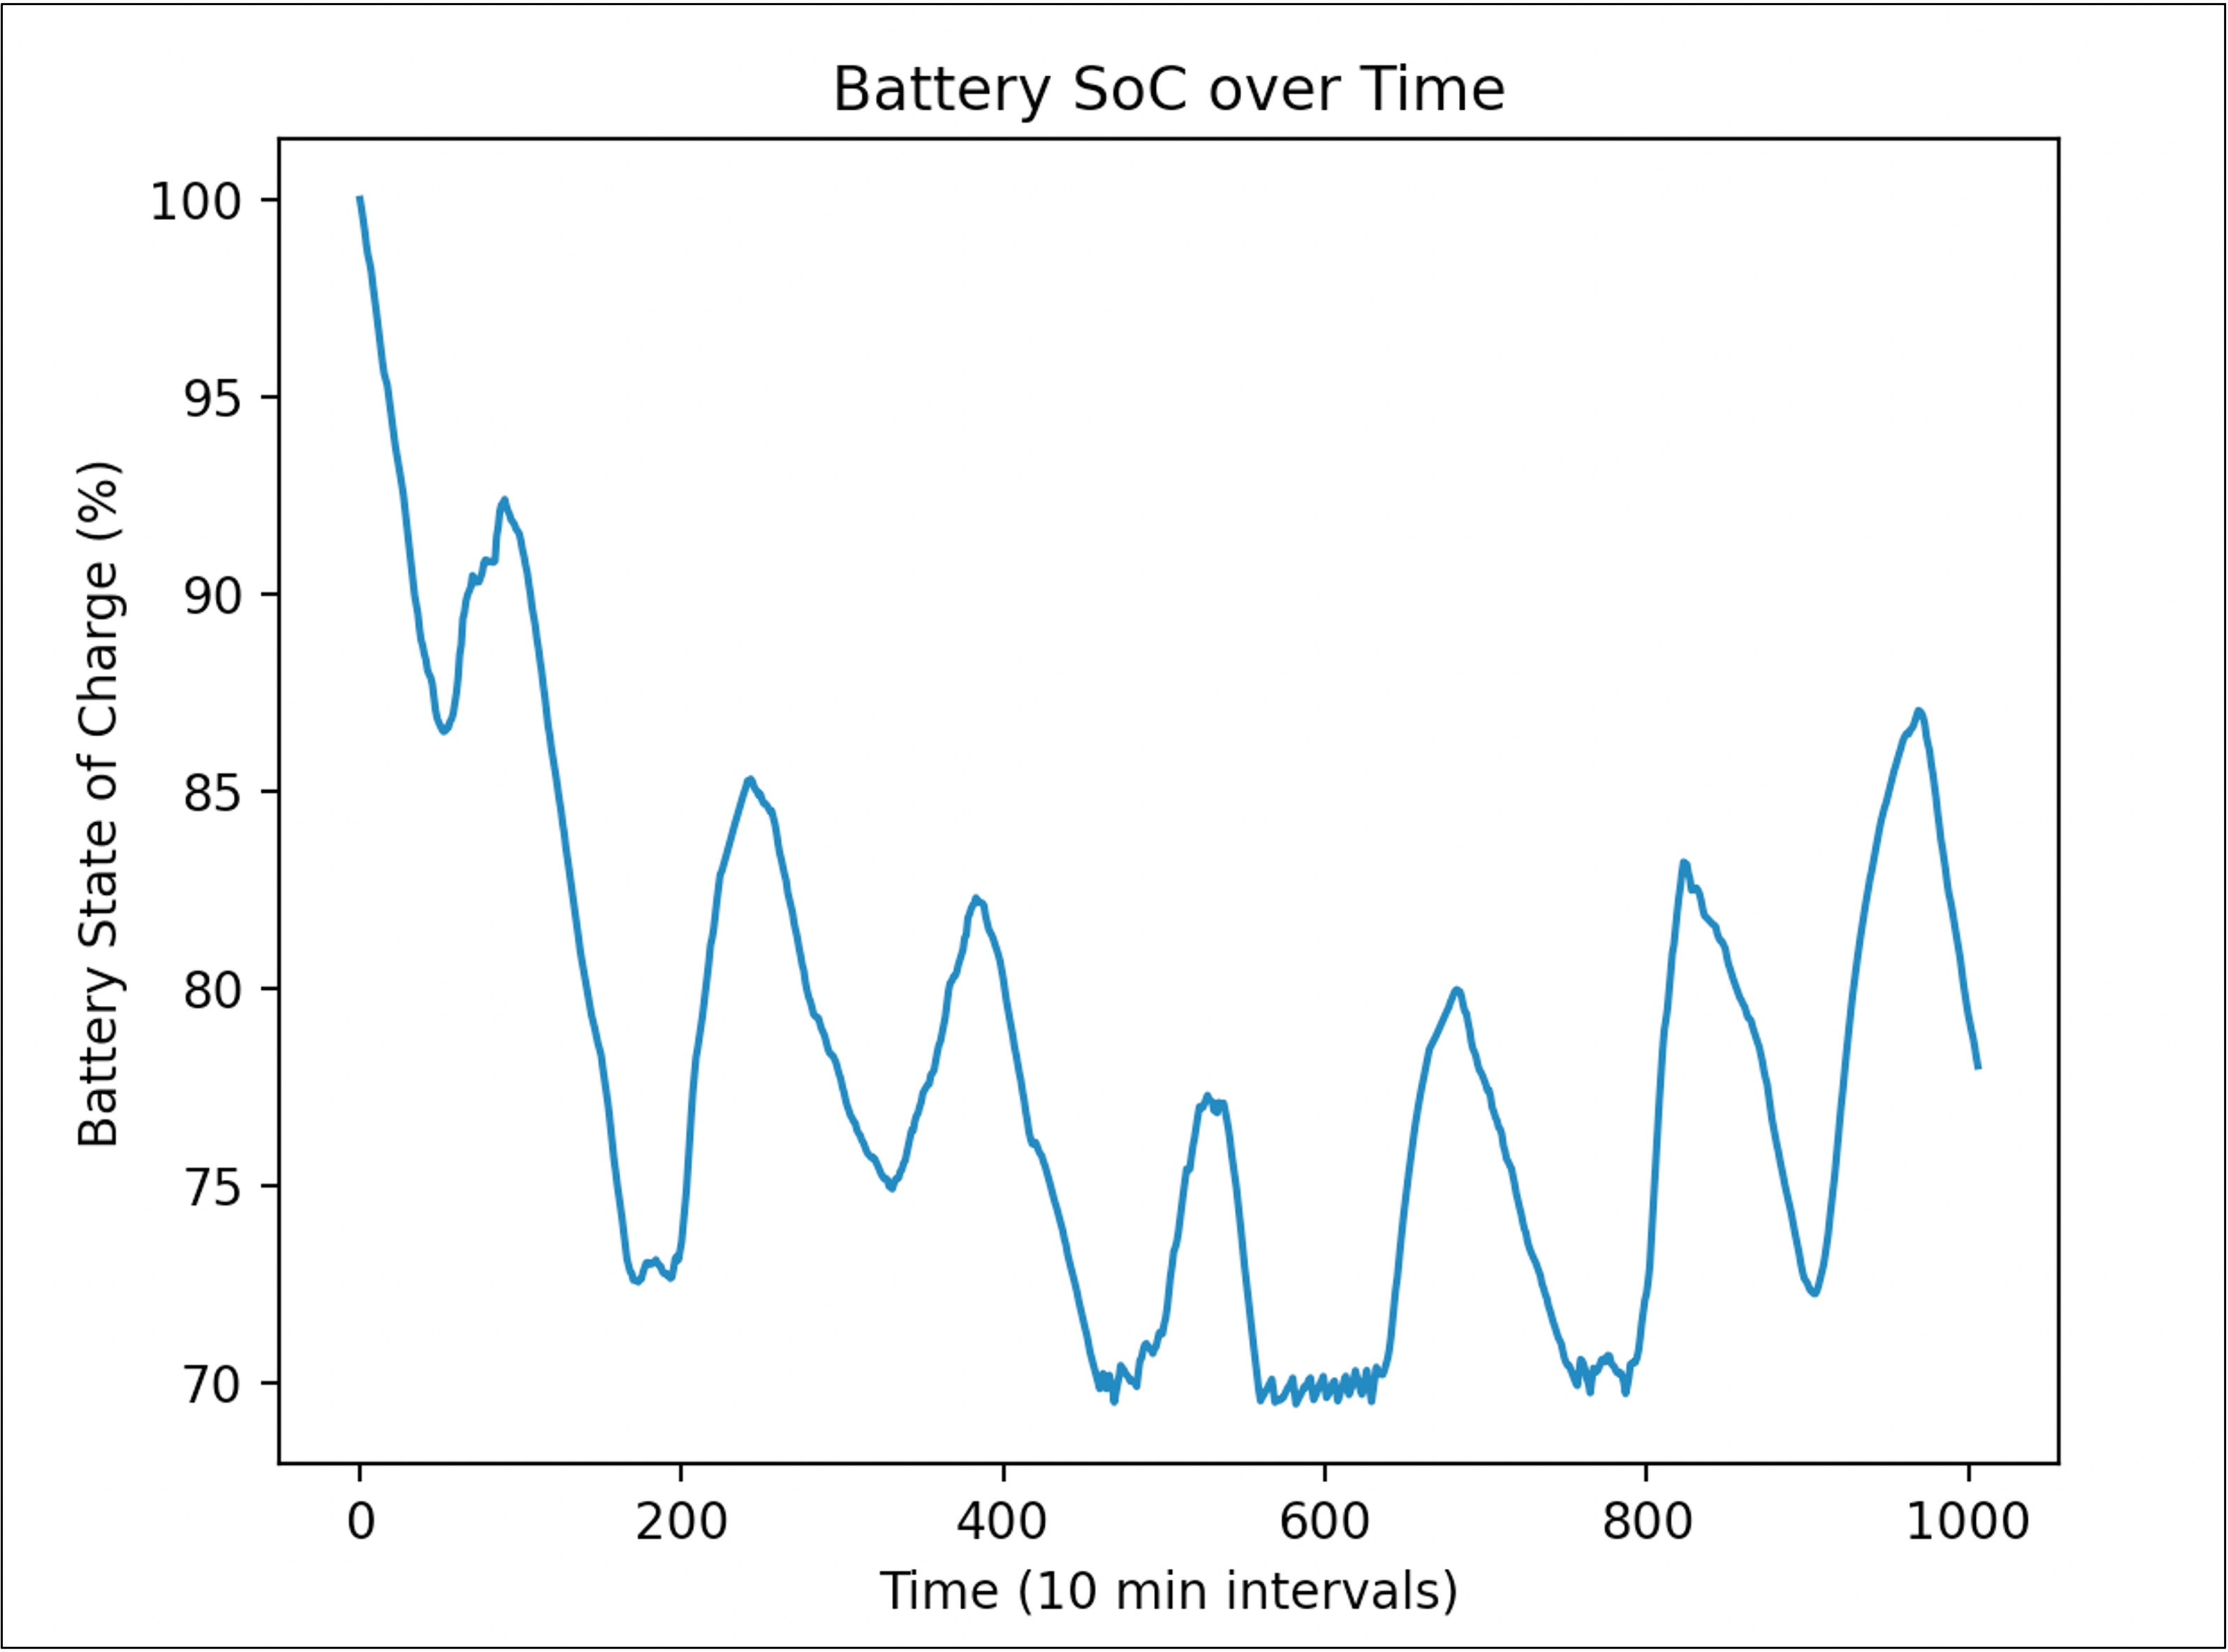
\includegraphics[width=\linewidth]{pics/naivesocvtime.jpg}
    \caption{SoC over time}
  \end{subfigure}
  \begin{subfigure}[b]{0.45\linewidth}
    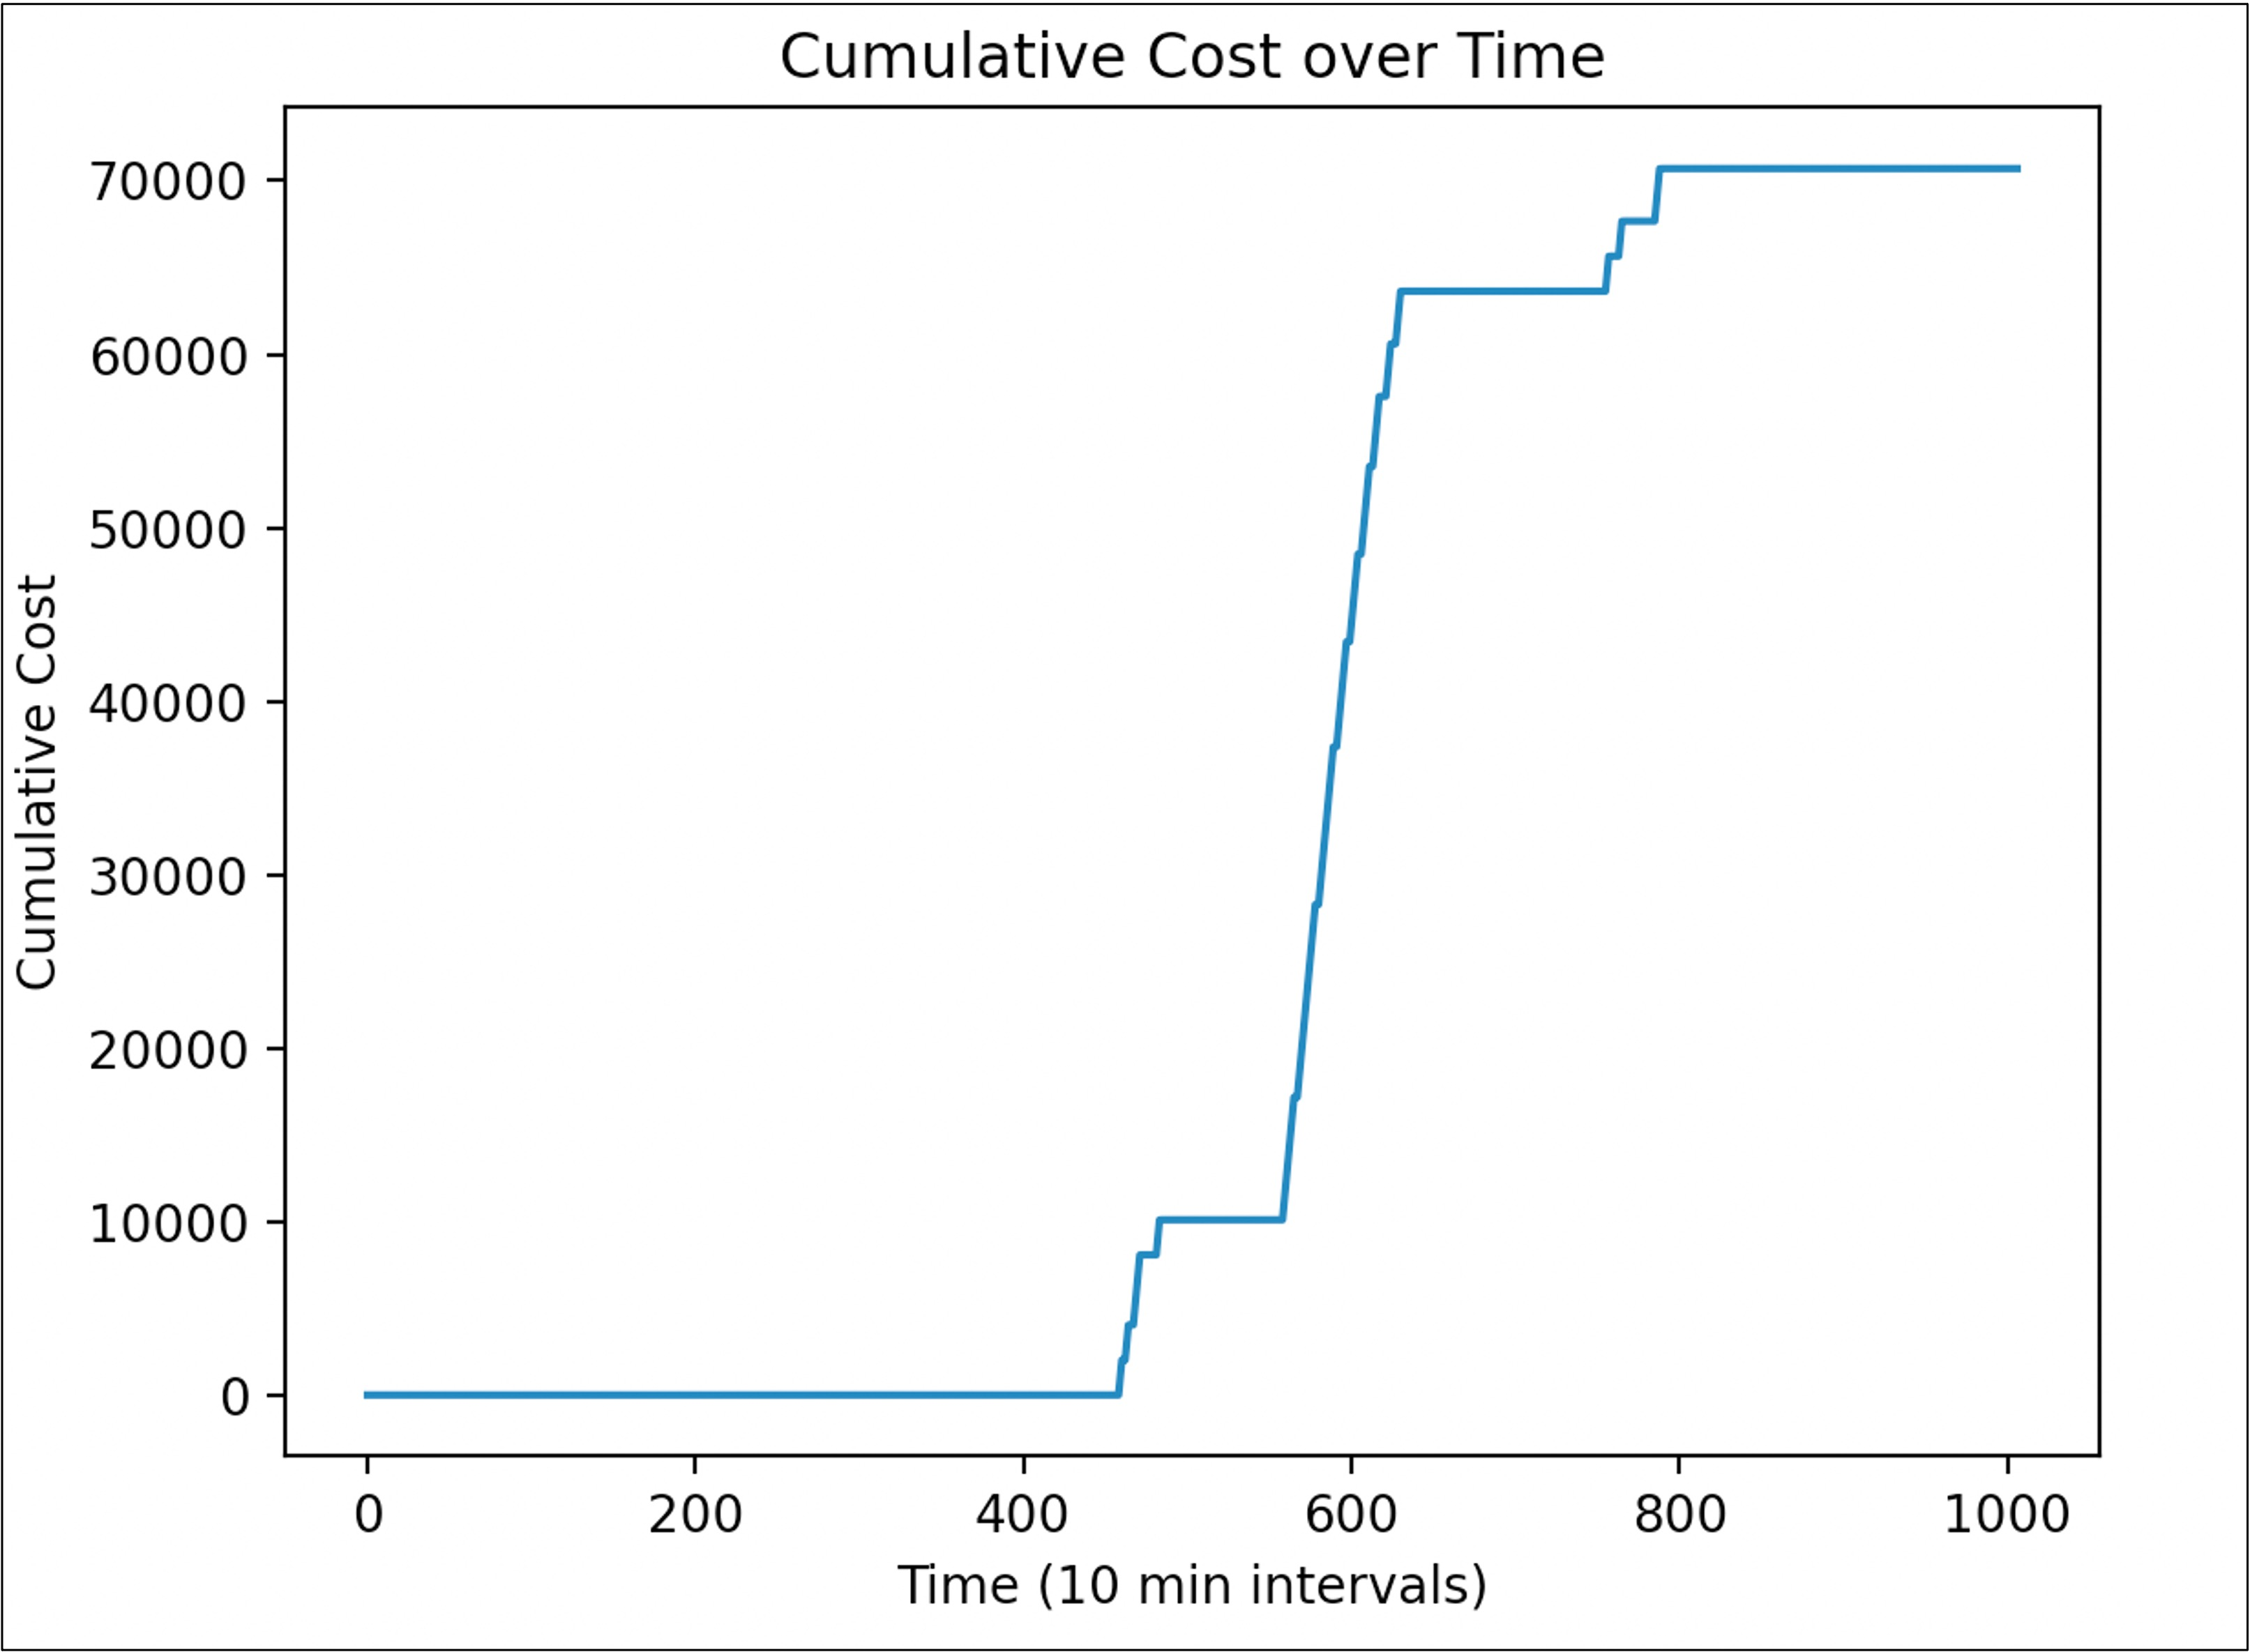
\includegraphics[width=\linewidth]{pics/naivecostvtime.jpg}
    \caption{Cumulative cost over time}
  \end{subfigure}
  \caption{Graphs from the naive SML policy}
  \label{fig:naive}
\end{figure}

\subsection{Linear Spline}

The linear spline model creates a piecewise linear function to approximate the value function. This produces the graph in Figure 2b. In Figure 2a, we see similar patterns to as what the naive policy produced, except that the SoC never drops below about 80\%. This is an improvement, because the battery bank lifespan will be degraded if the SoC drops below about 70\%. The value function approximation in Figure 2b also provides interesting insights. The function trends upwards for higher SoC values, which intuitively makes sense, higher battery charge is a good thing. However, the value function has a strange pattern below 50\% SoC, where it increases again as SoC decreases. This pattern is likely caused by a lack of training data in the region below 50\% SoC. Its also apparent that the model values running the generator more at lower SoC values, because the red line is higher than the green line for lower SoC values. This matches the intuition of the problem because there is no need to run the generator if the battery has a high SoC. In Figure 2c, the cumulative cost is graphed. This plot shows a similar pattern to the naive policy in Figure 1b, but with a significantly lower total cost of about 1000. This is an improvement over the naive policy in simulation.

\begin{figure}[H]
  \centering
  \begin{subfigure}[b]{0.3\linewidth}
    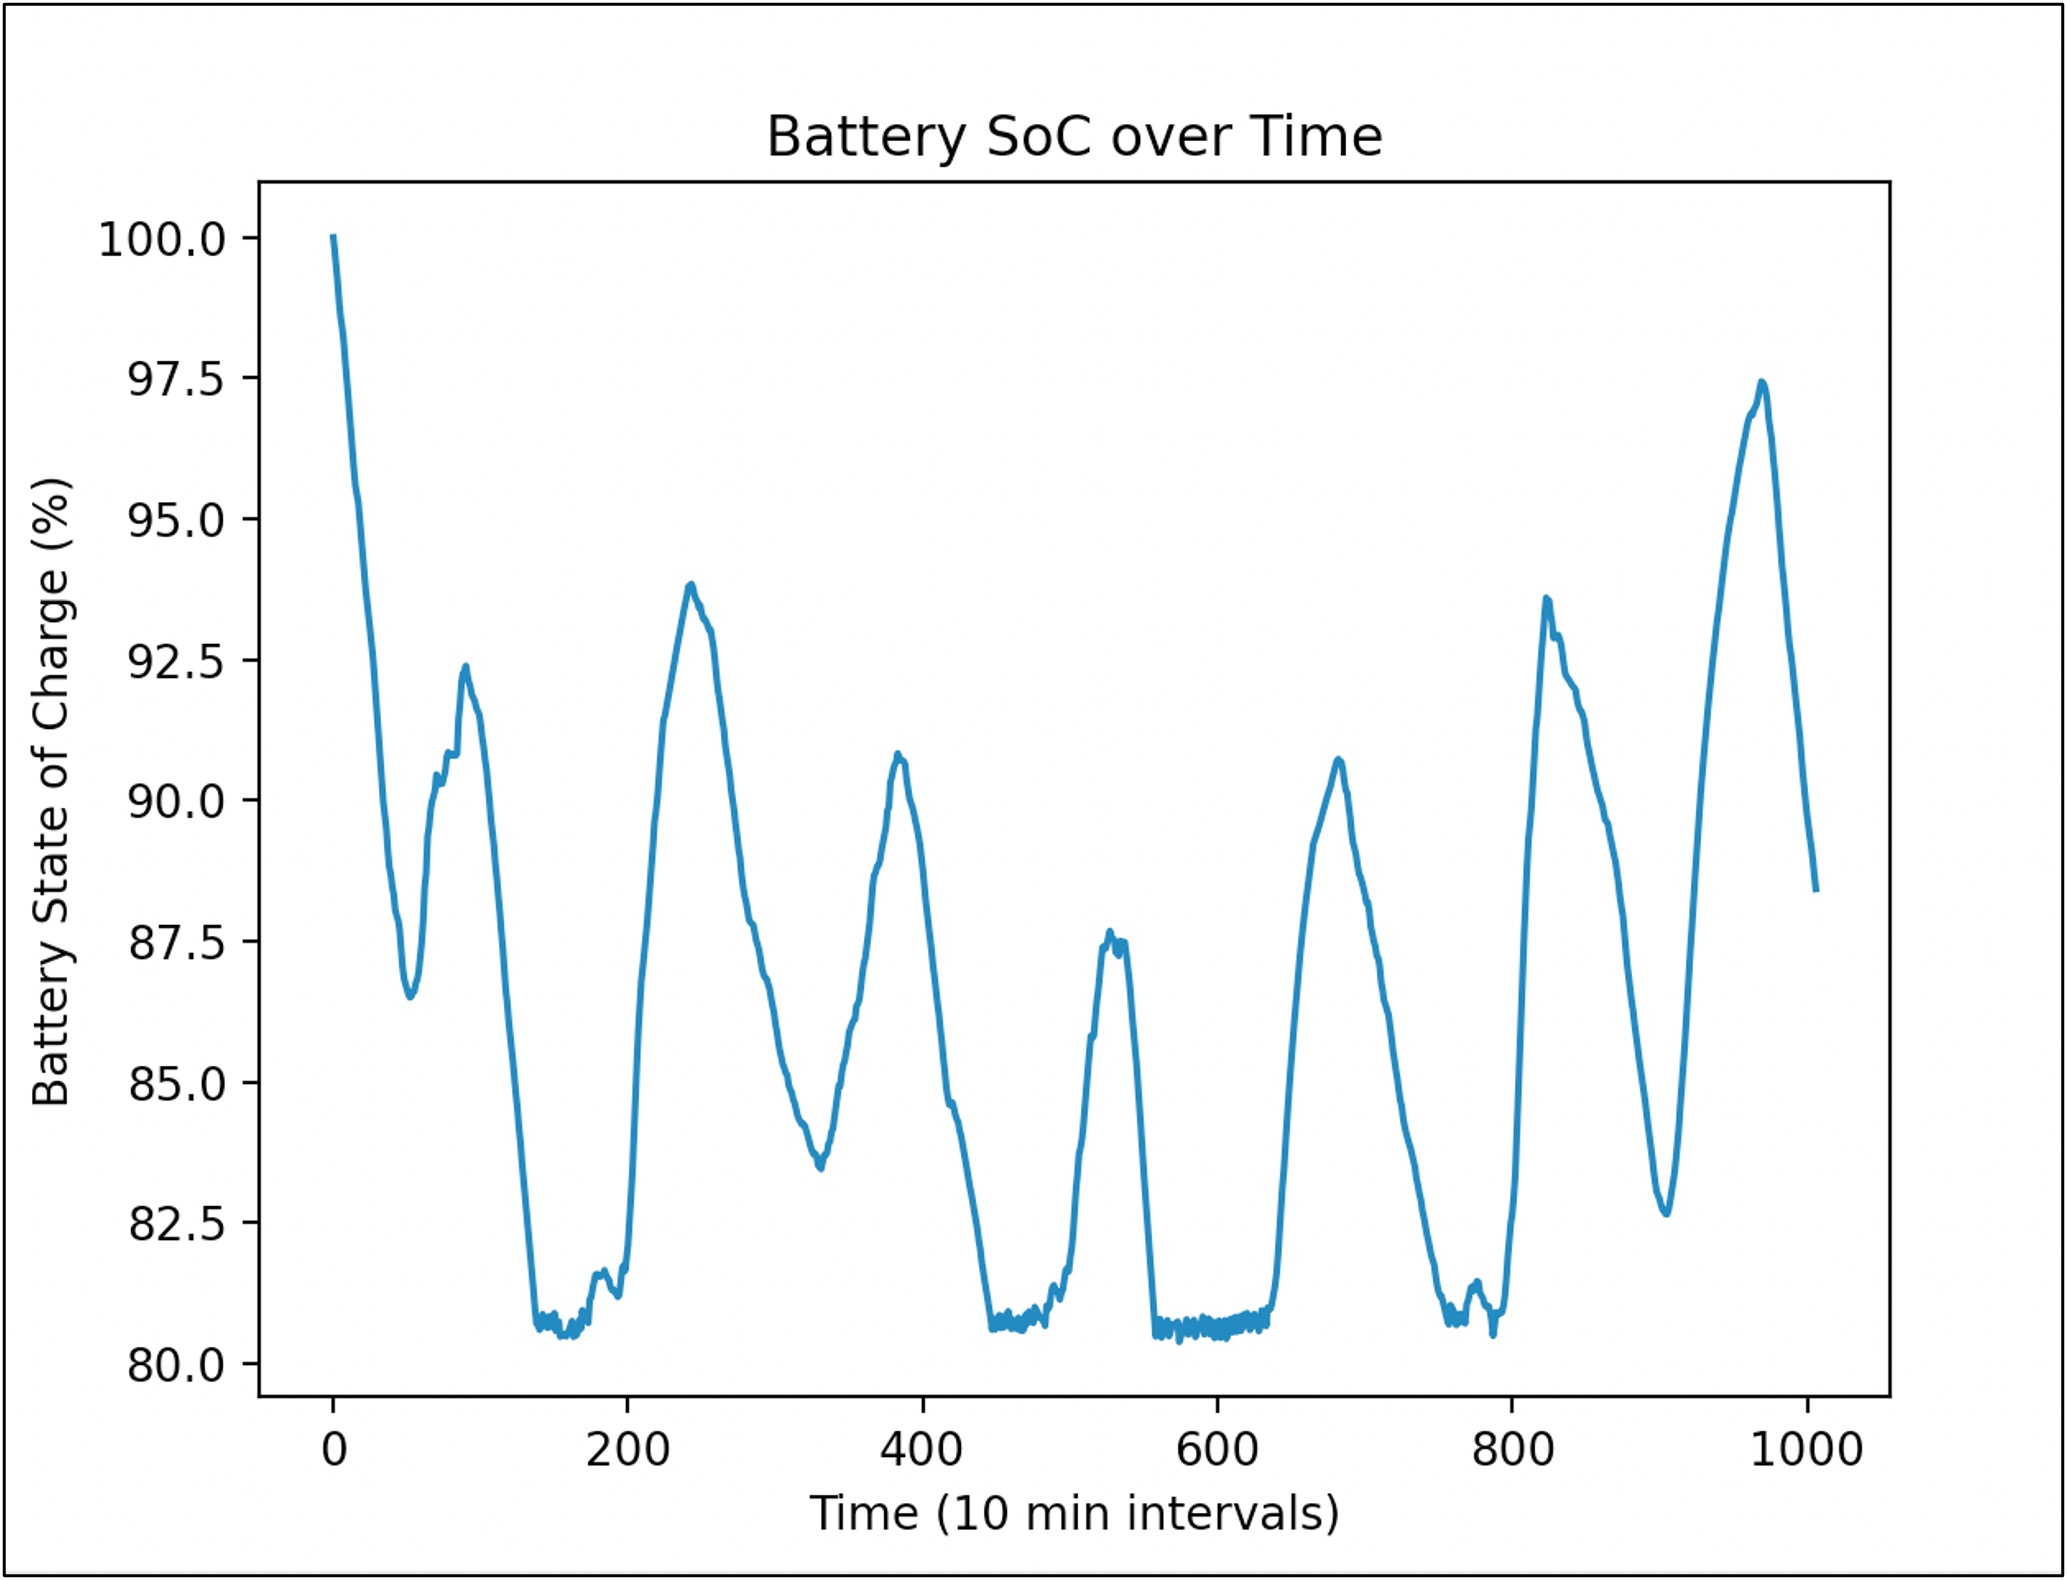
\includegraphics[width=\linewidth]{pics/linsocvtime.jpg}
    \caption{SoC over time}
  \end{subfigure}
  \begin{subfigure}[b]{0.3\linewidth}
    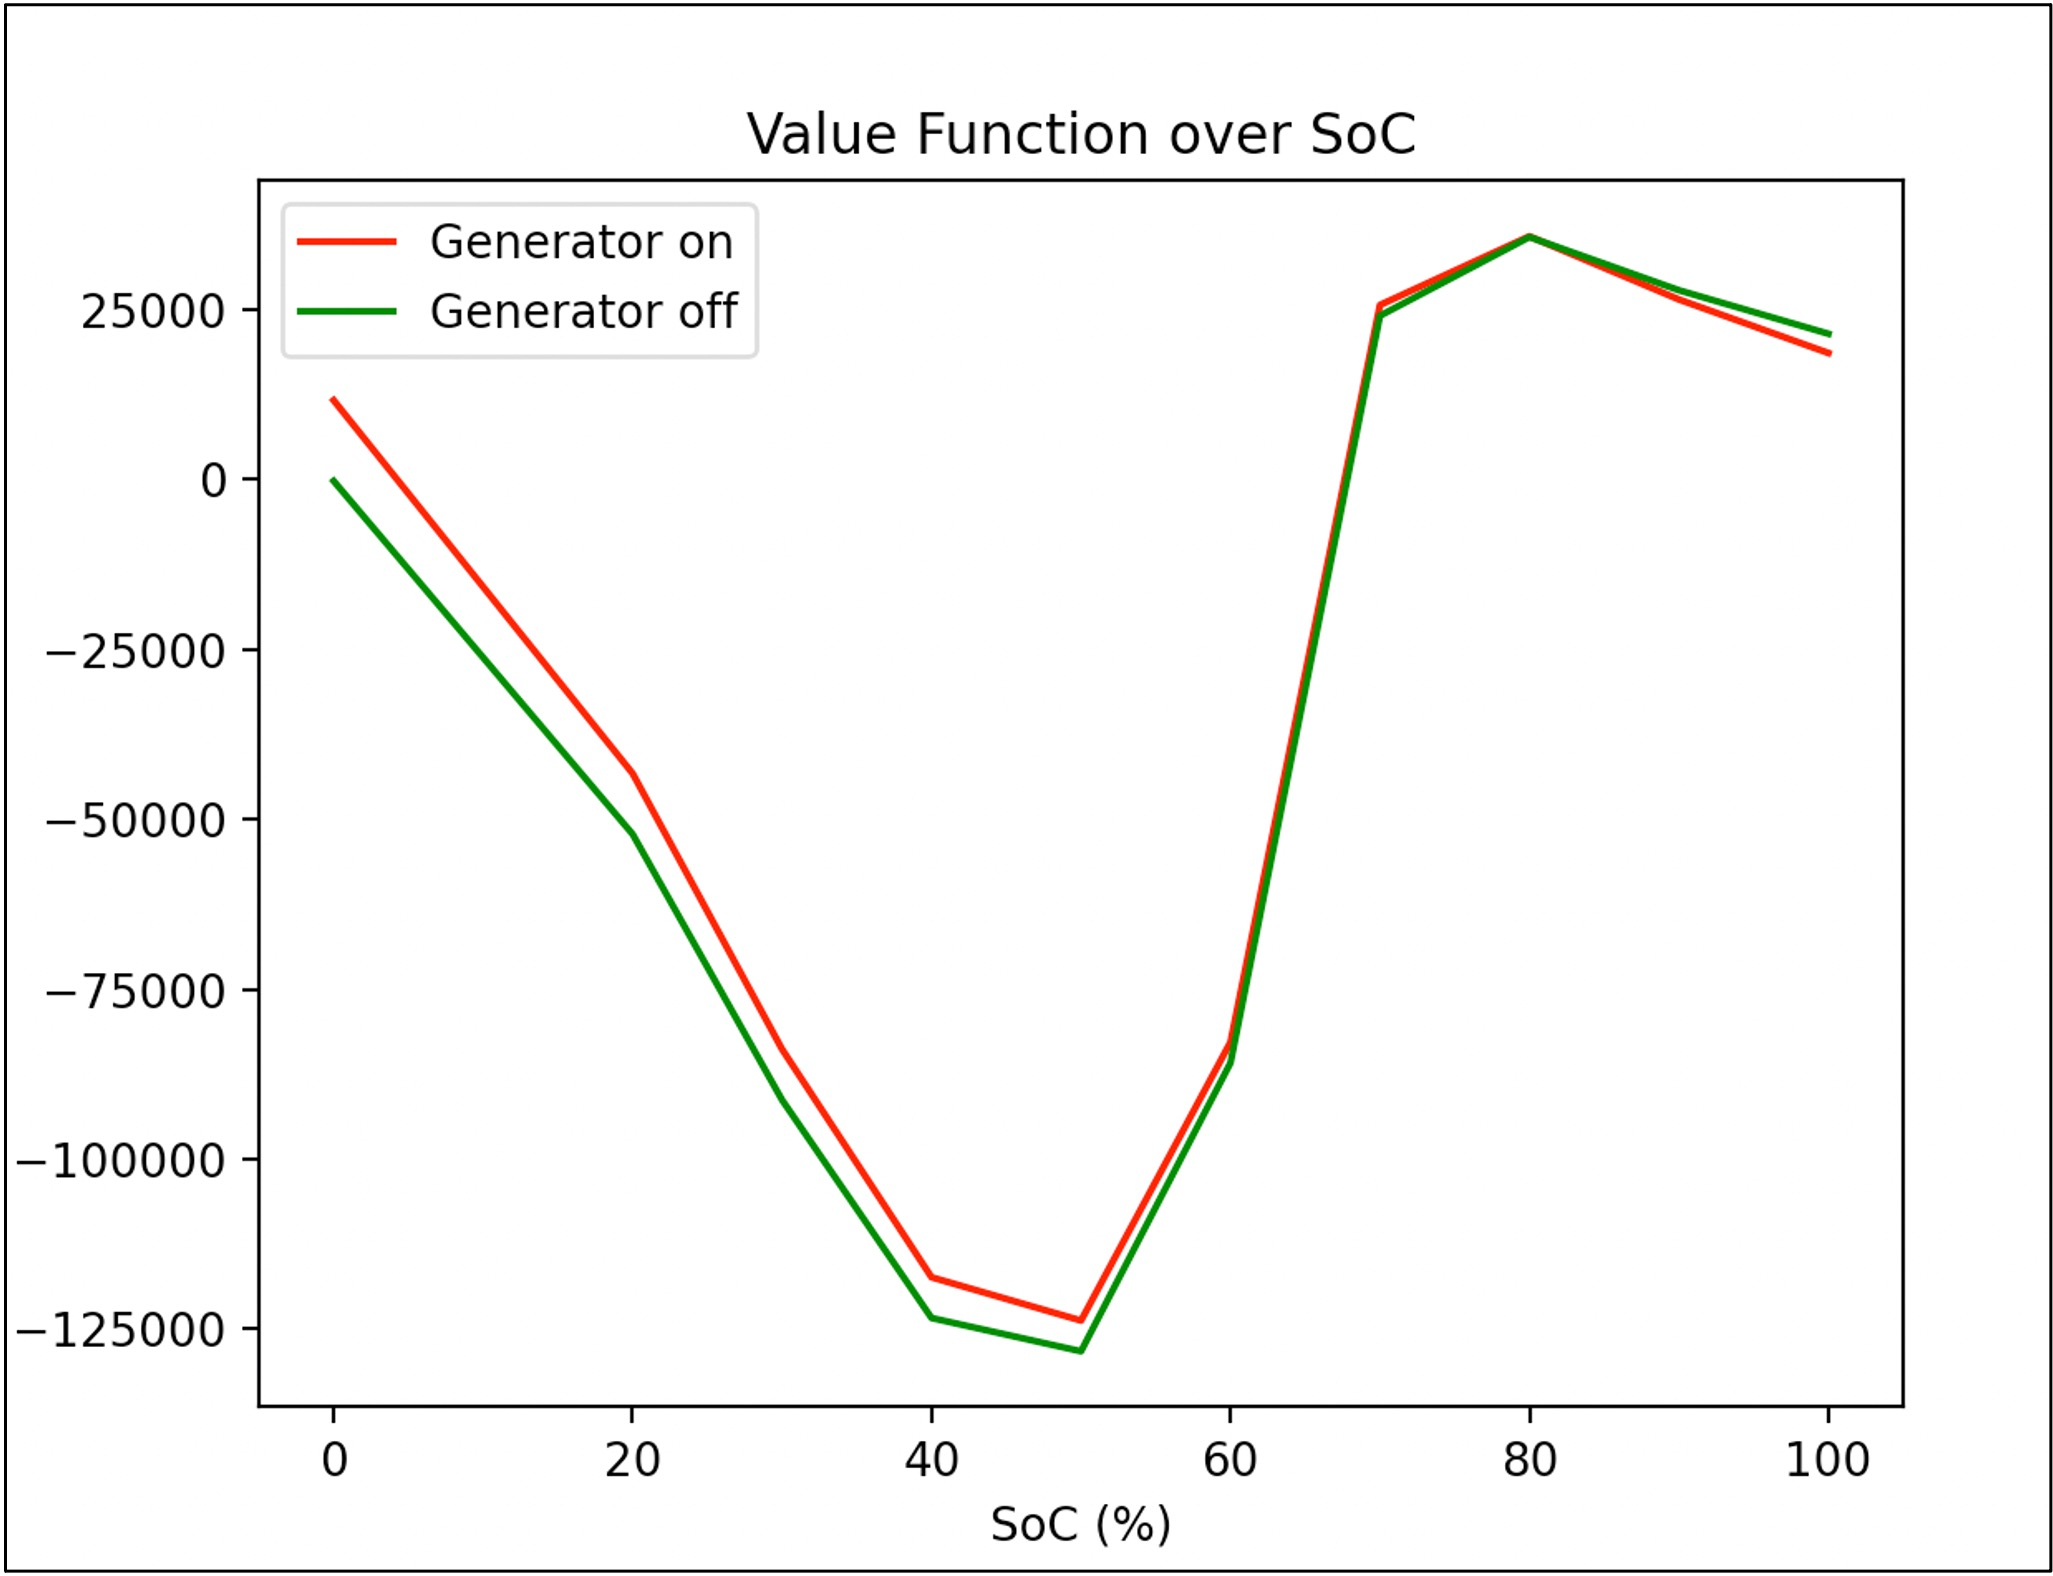
\includegraphics[width=\linewidth]{pics/linvaluefunc.jpg}
    \caption{Value function approximation}
  \end{subfigure}
  \begin{subfigure}[b]{0.3\linewidth}
    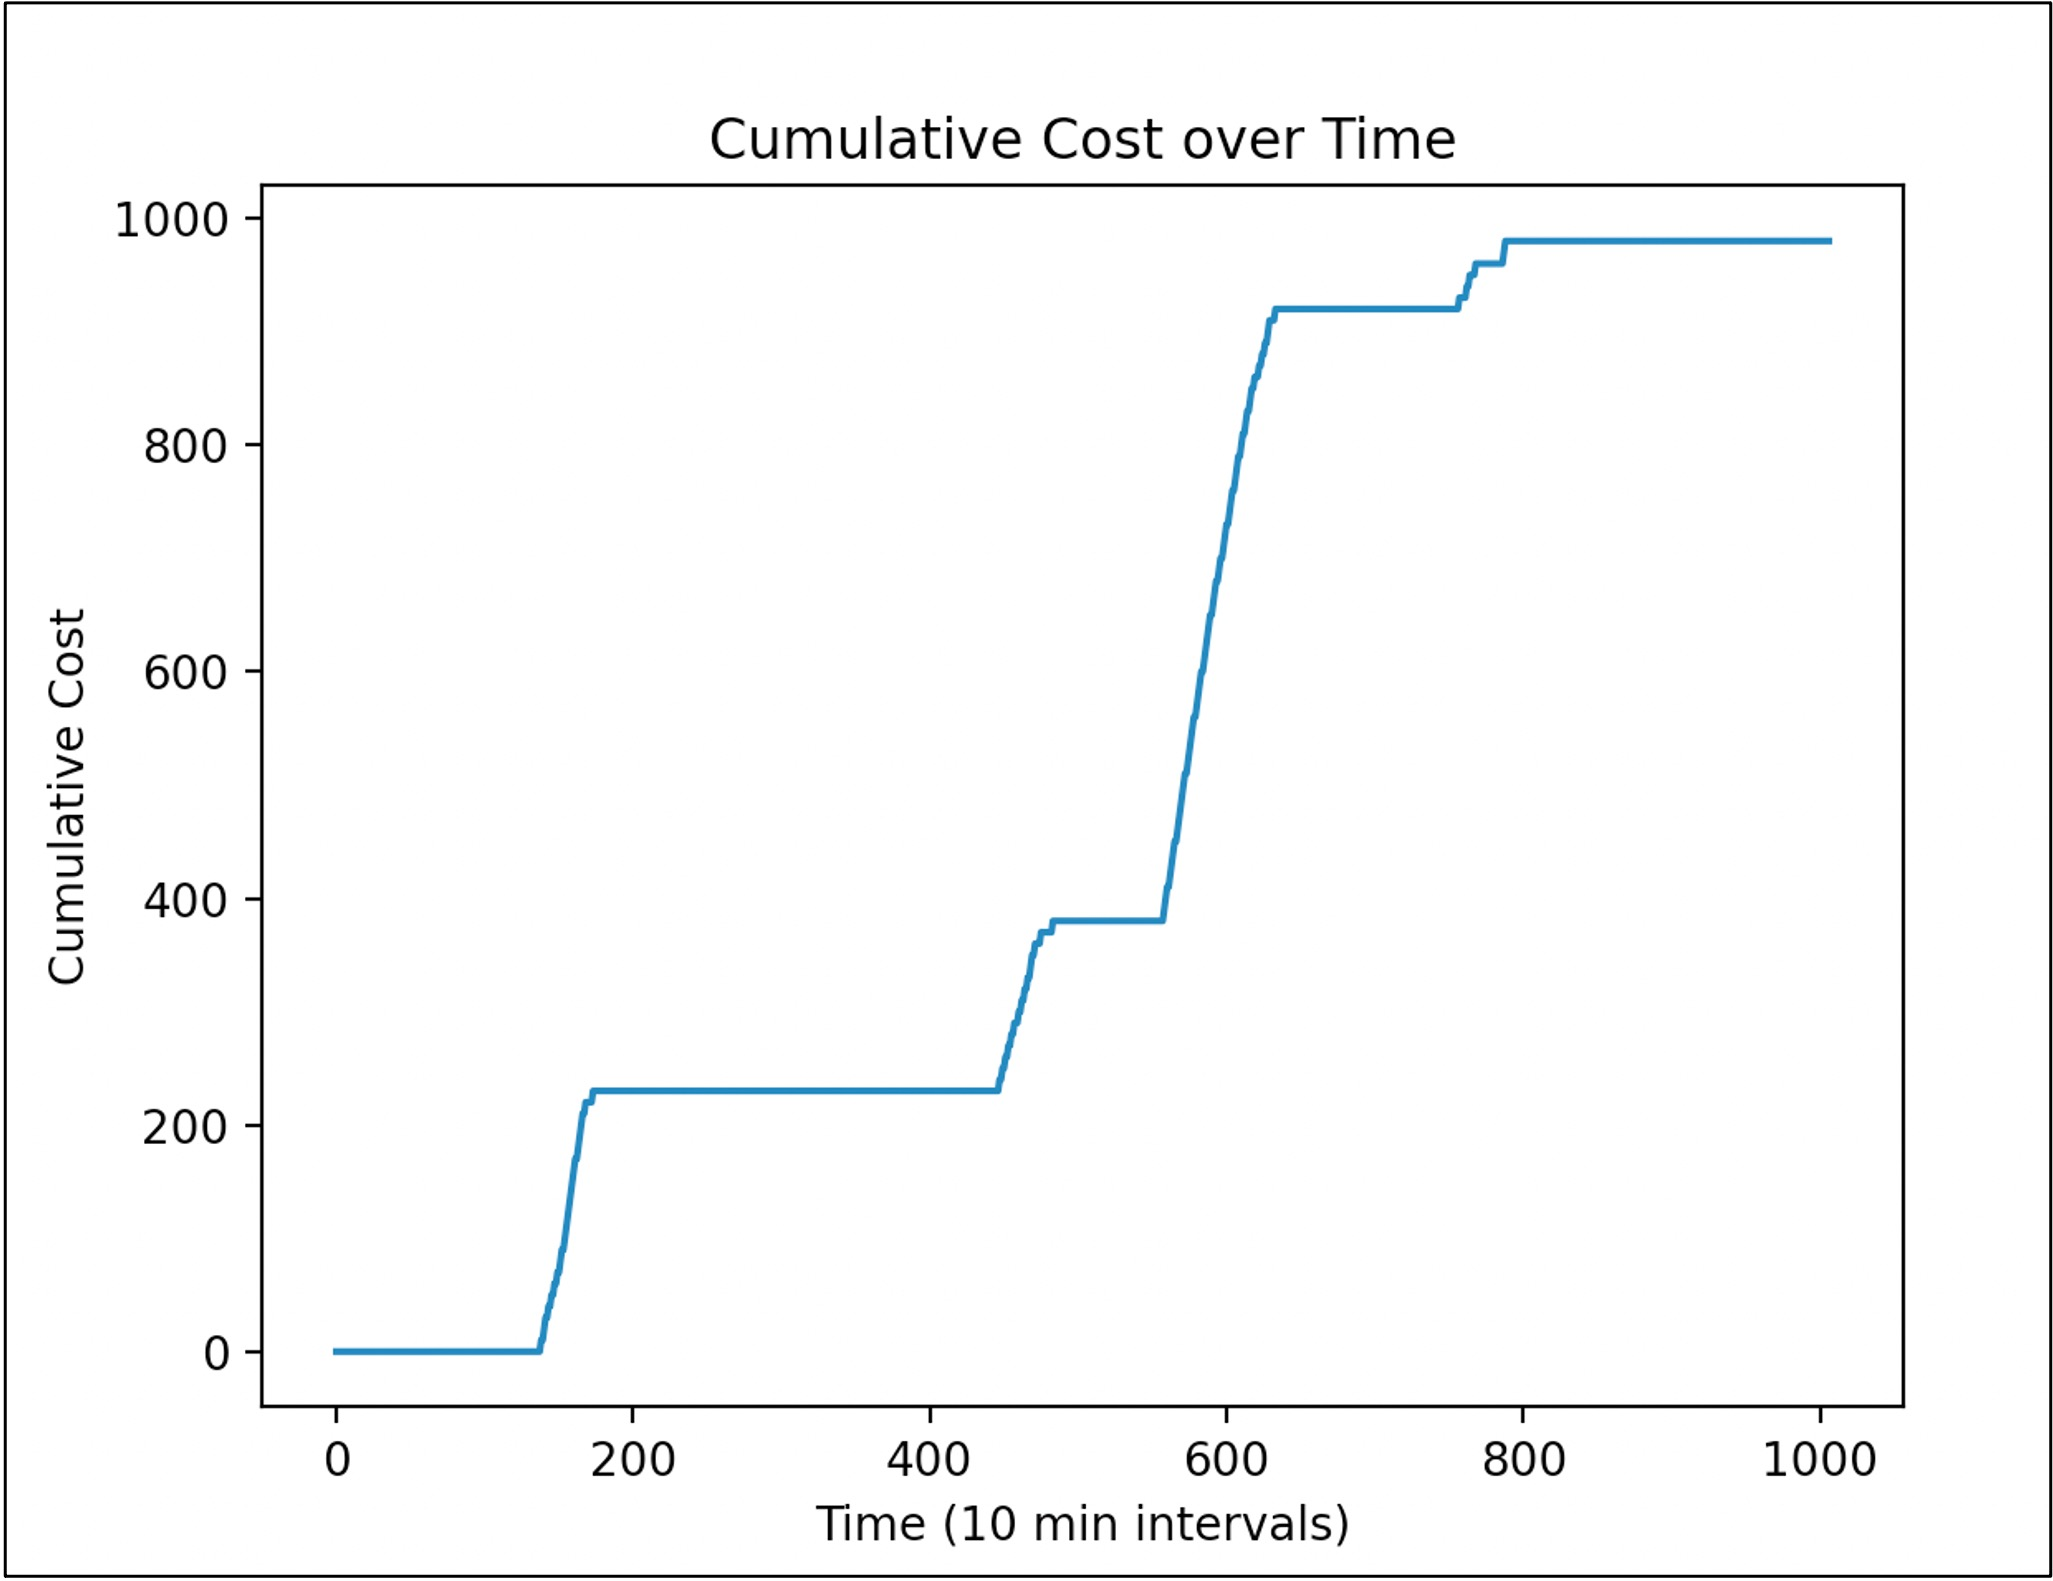
\includegraphics[width=\linewidth]{pics/lincostvtime.jpg}
    \caption{Cumulative cost over time}
  \end{subfigure}
  \caption{Graphs from the linear spline model's policy}
  \label{fig:linearspline}
\end{figure}

\subsection{Neural Network}

The NN model produced an approximation of the value function, shown in Figure 3b. This model was trained on one day of data due to computation time constraints and had lackluster results. The graph of SoC in Figure 3a shows that the battery was almost never discharged because the lowest value is 99.75\%. In the value function approximation in Figure 3b, we can see an upward trend similar to the linear spline model, but where the generator being on is preferred for nearly all SoC values. This is problematic, and probably explains why the battery never discharged below 99\%. In Figure 3c, the cumulative cost appears to be linear. This means the agent was constantly incurring cost. Since the SoC never got low, this shows that the agent decided to constantly run the generator. For obvious reasons, this model is not very successful or practical.

The issues with the NN model could be caused by multiple factors. The first is the lack of training time. This model was very time intensive to train, so only one day of data was used. This likely wasn't enough time for the model to get a good fit of the value function. Also, the configuration of the NN could have been suboptimal for this problem. A simplistic NN with no hidden layers was used. The NN had two input nodes (one for current SoC value and one for if the generators are currently running) and one output node for the value function output. With further tuning and more training time, it is possible the NN model could have produced better results.

\begin{figure}[H]
  \centering
  \begin{subfigure}[b]{0.3\linewidth}
    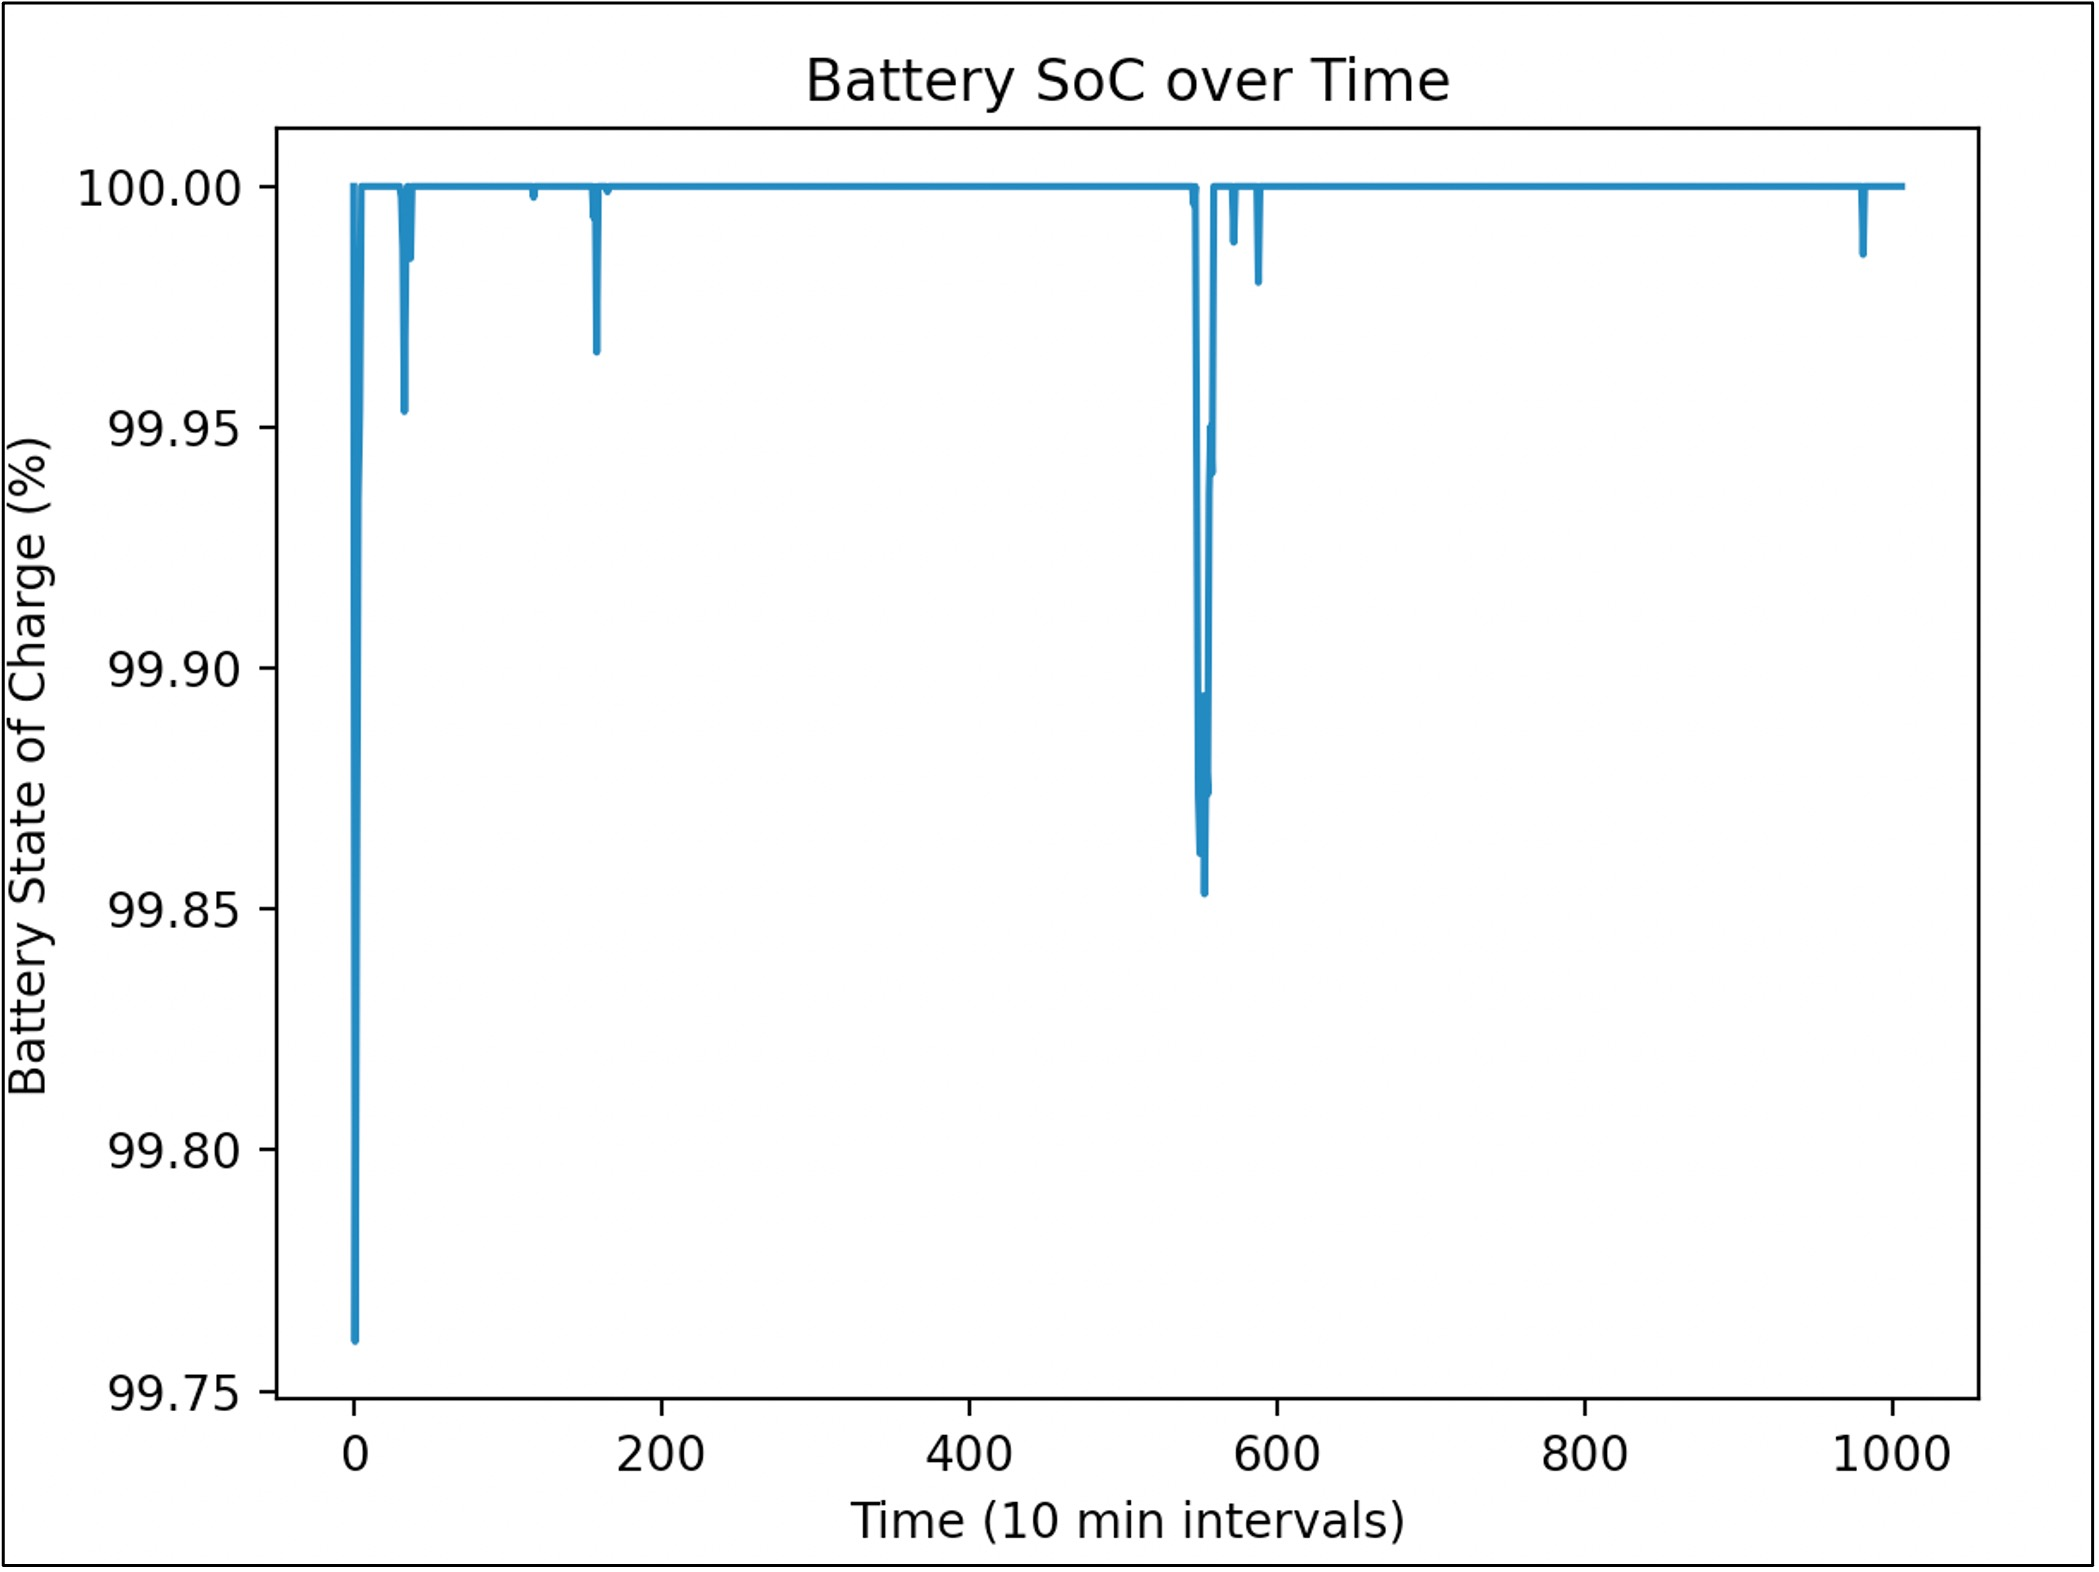
\includegraphics[width=\linewidth]{pics/nnsocvtime.jpg}
    \caption{SoC over time}
  \end{subfigure}
  \begin{subfigure}[b]{0.3\linewidth}
    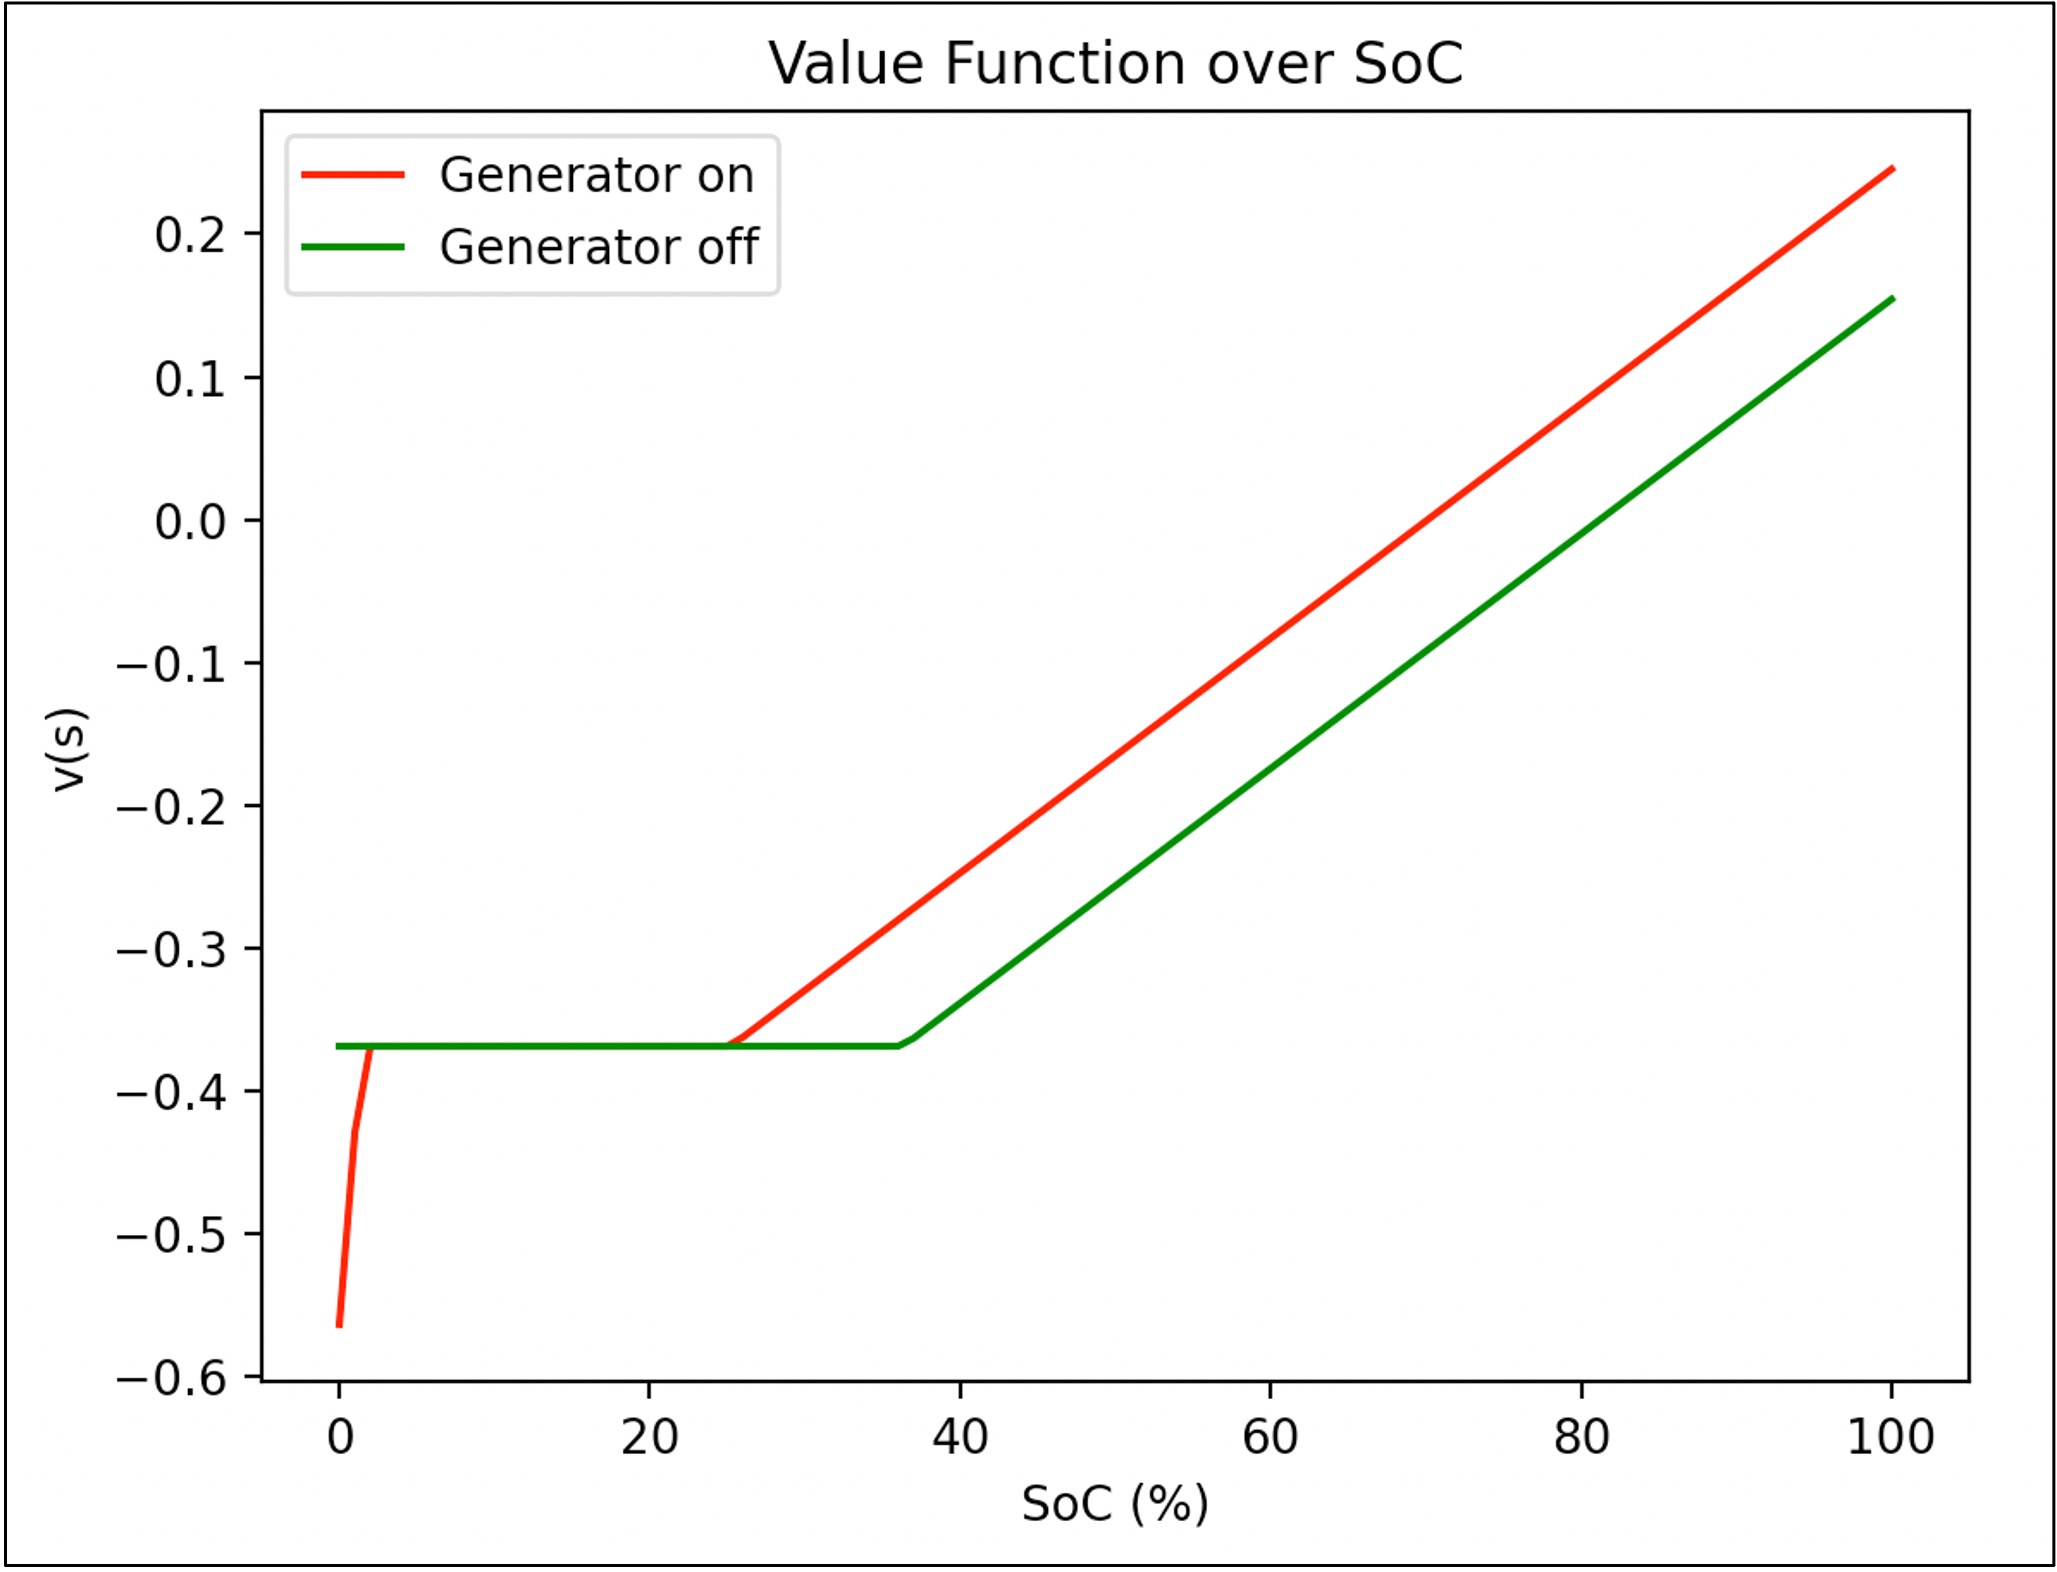
\includegraphics[width=\linewidth]{pics/nnvaluefunc.jpg}
    \caption{Value function approximation}
  \end{subfigure}
  \begin{subfigure}[b]{0.3\linewidth}
    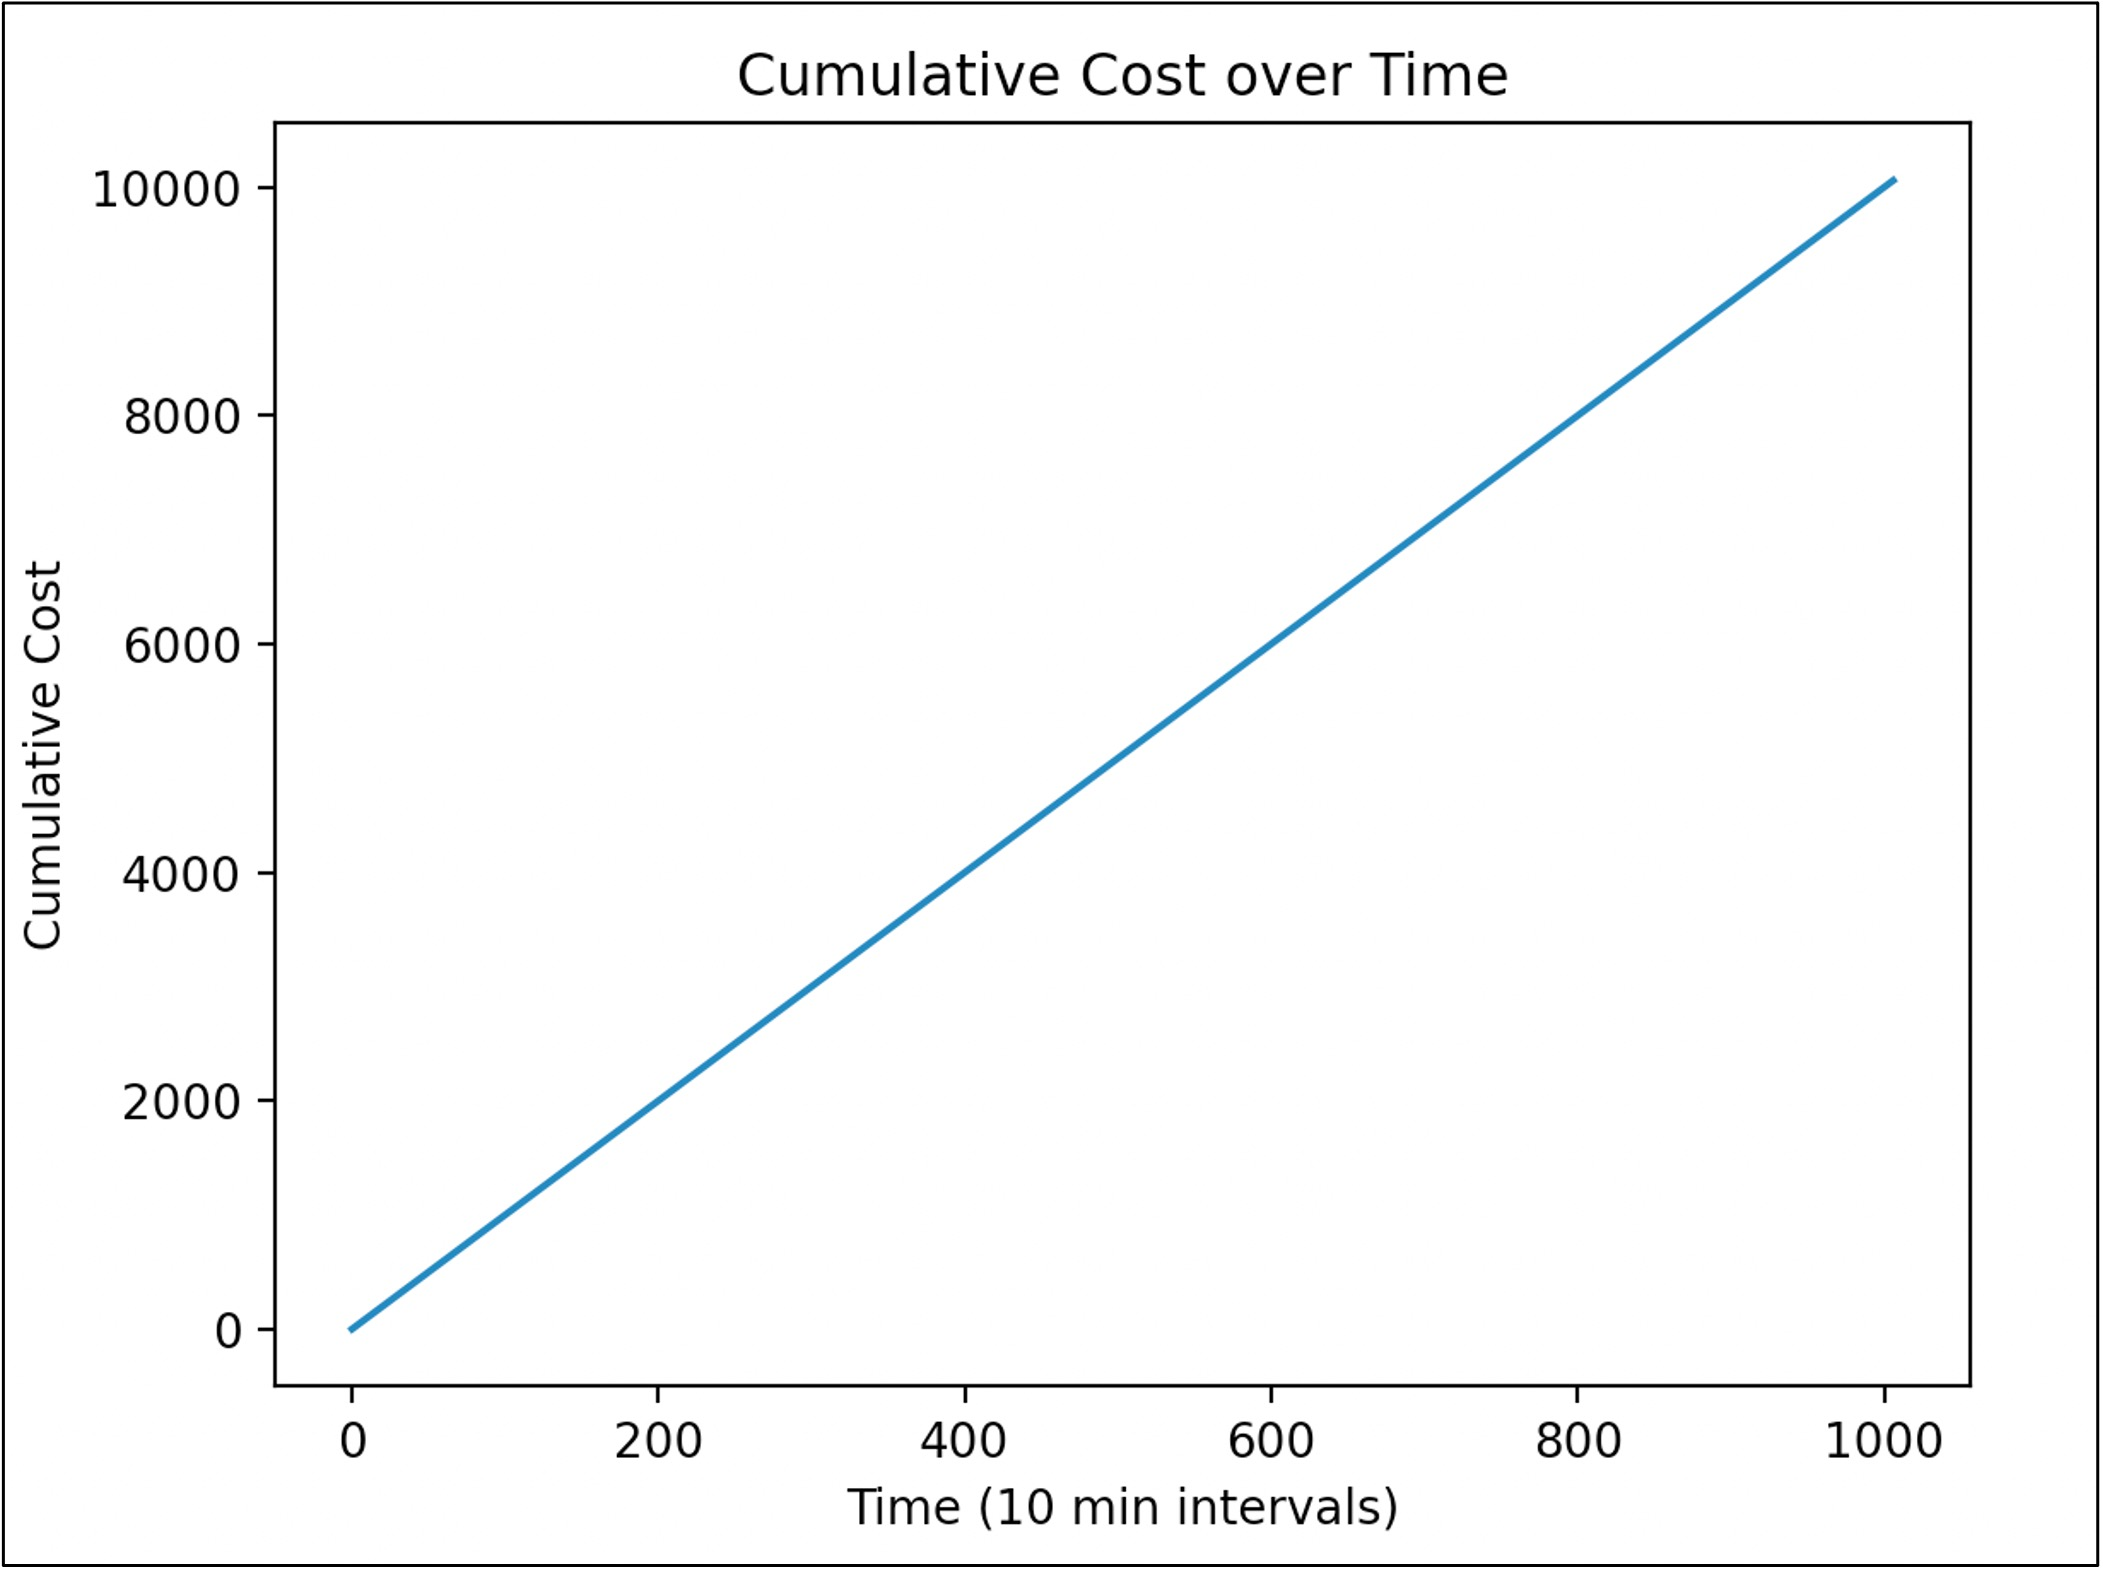
\includegraphics[width=\linewidth]{pics/nncostvtime.jpg}
    \caption{Cumulative cost over time}
  \end{subfigure}
  \caption{Graphs from the NN model's policy}
  \label{fig:nngraphs}
\end{figure}

\subsection{Radial Basis Function}

The RBF model fits a nonlinear function to approximate the value function. It resulted in a a similar SoC graph as the linear spline model, shown in Figure 4a. There are the same day and night patterns as solar energy becomes available, with the battery SoC hitting a minimum of around 75\%. The value function approximation is shown in Figure 4b. This resulted in a curve with one valley, centered at around 40\% SoC. It is likely this approximation had a similar obstacles as the linear spline, where the a lack of training data for low SoC values caused a poor fit. This is why the curve has high values for low SoC. It is also strange that there is no clear difference between states with the generators on or off, because the green and red lines are overlapping. This characteristic would likely lead to issues in the policy. Lastly, the lack of differences between values above about 60\% SoC is concerning. According to the plot, having 60\% SoC and 100\% SoC are of the same value. This could lead to issues with battery degradation in practice. The cumulative cost shown in Figure 4c, there is a similar pattern to the linear spline model. One key difference is that the final value is actually the lowest of the 4 policies tested in simulation, with a value around 800. The RBF model has great potential, but the issues mentioned here make the linear spline model a more robust choice.

\begin{figure}[H]
  \centering
  \begin{subfigure}[b]{0.3\linewidth}
    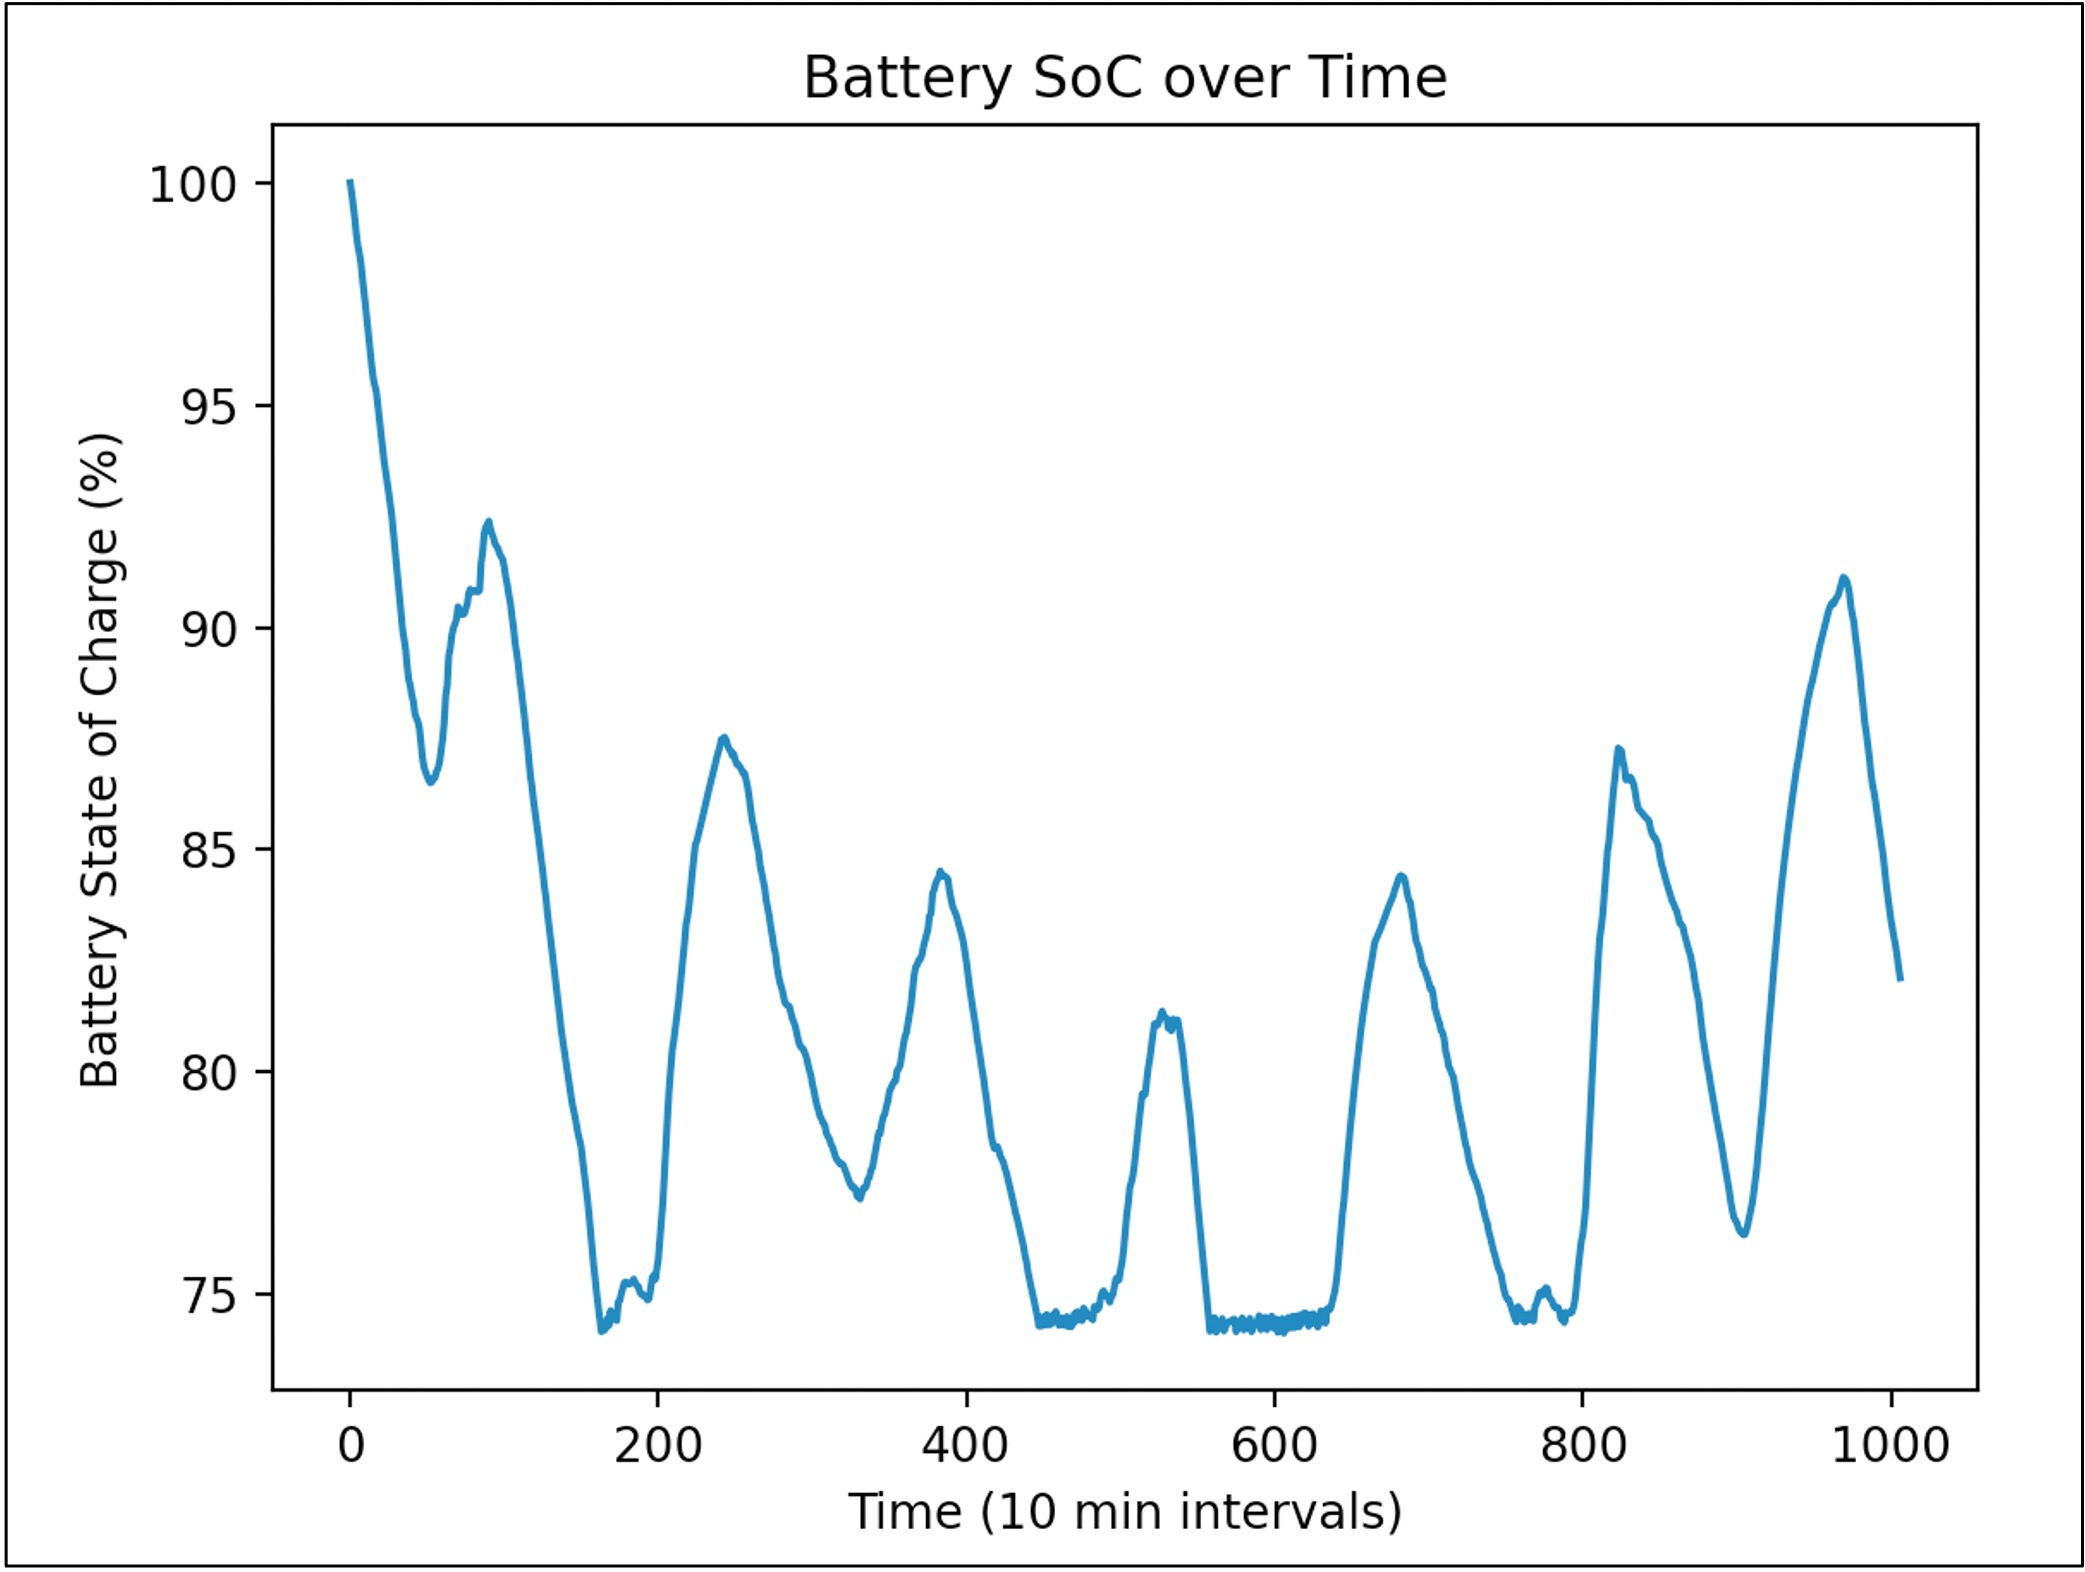
\includegraphics[width=\linewidth]{pics/rbfsocvtime.jpg}
    \caption{SoC over time}
  \end{subfigure}
  \begin{subfigure}[b]{0.3\linewidth}
    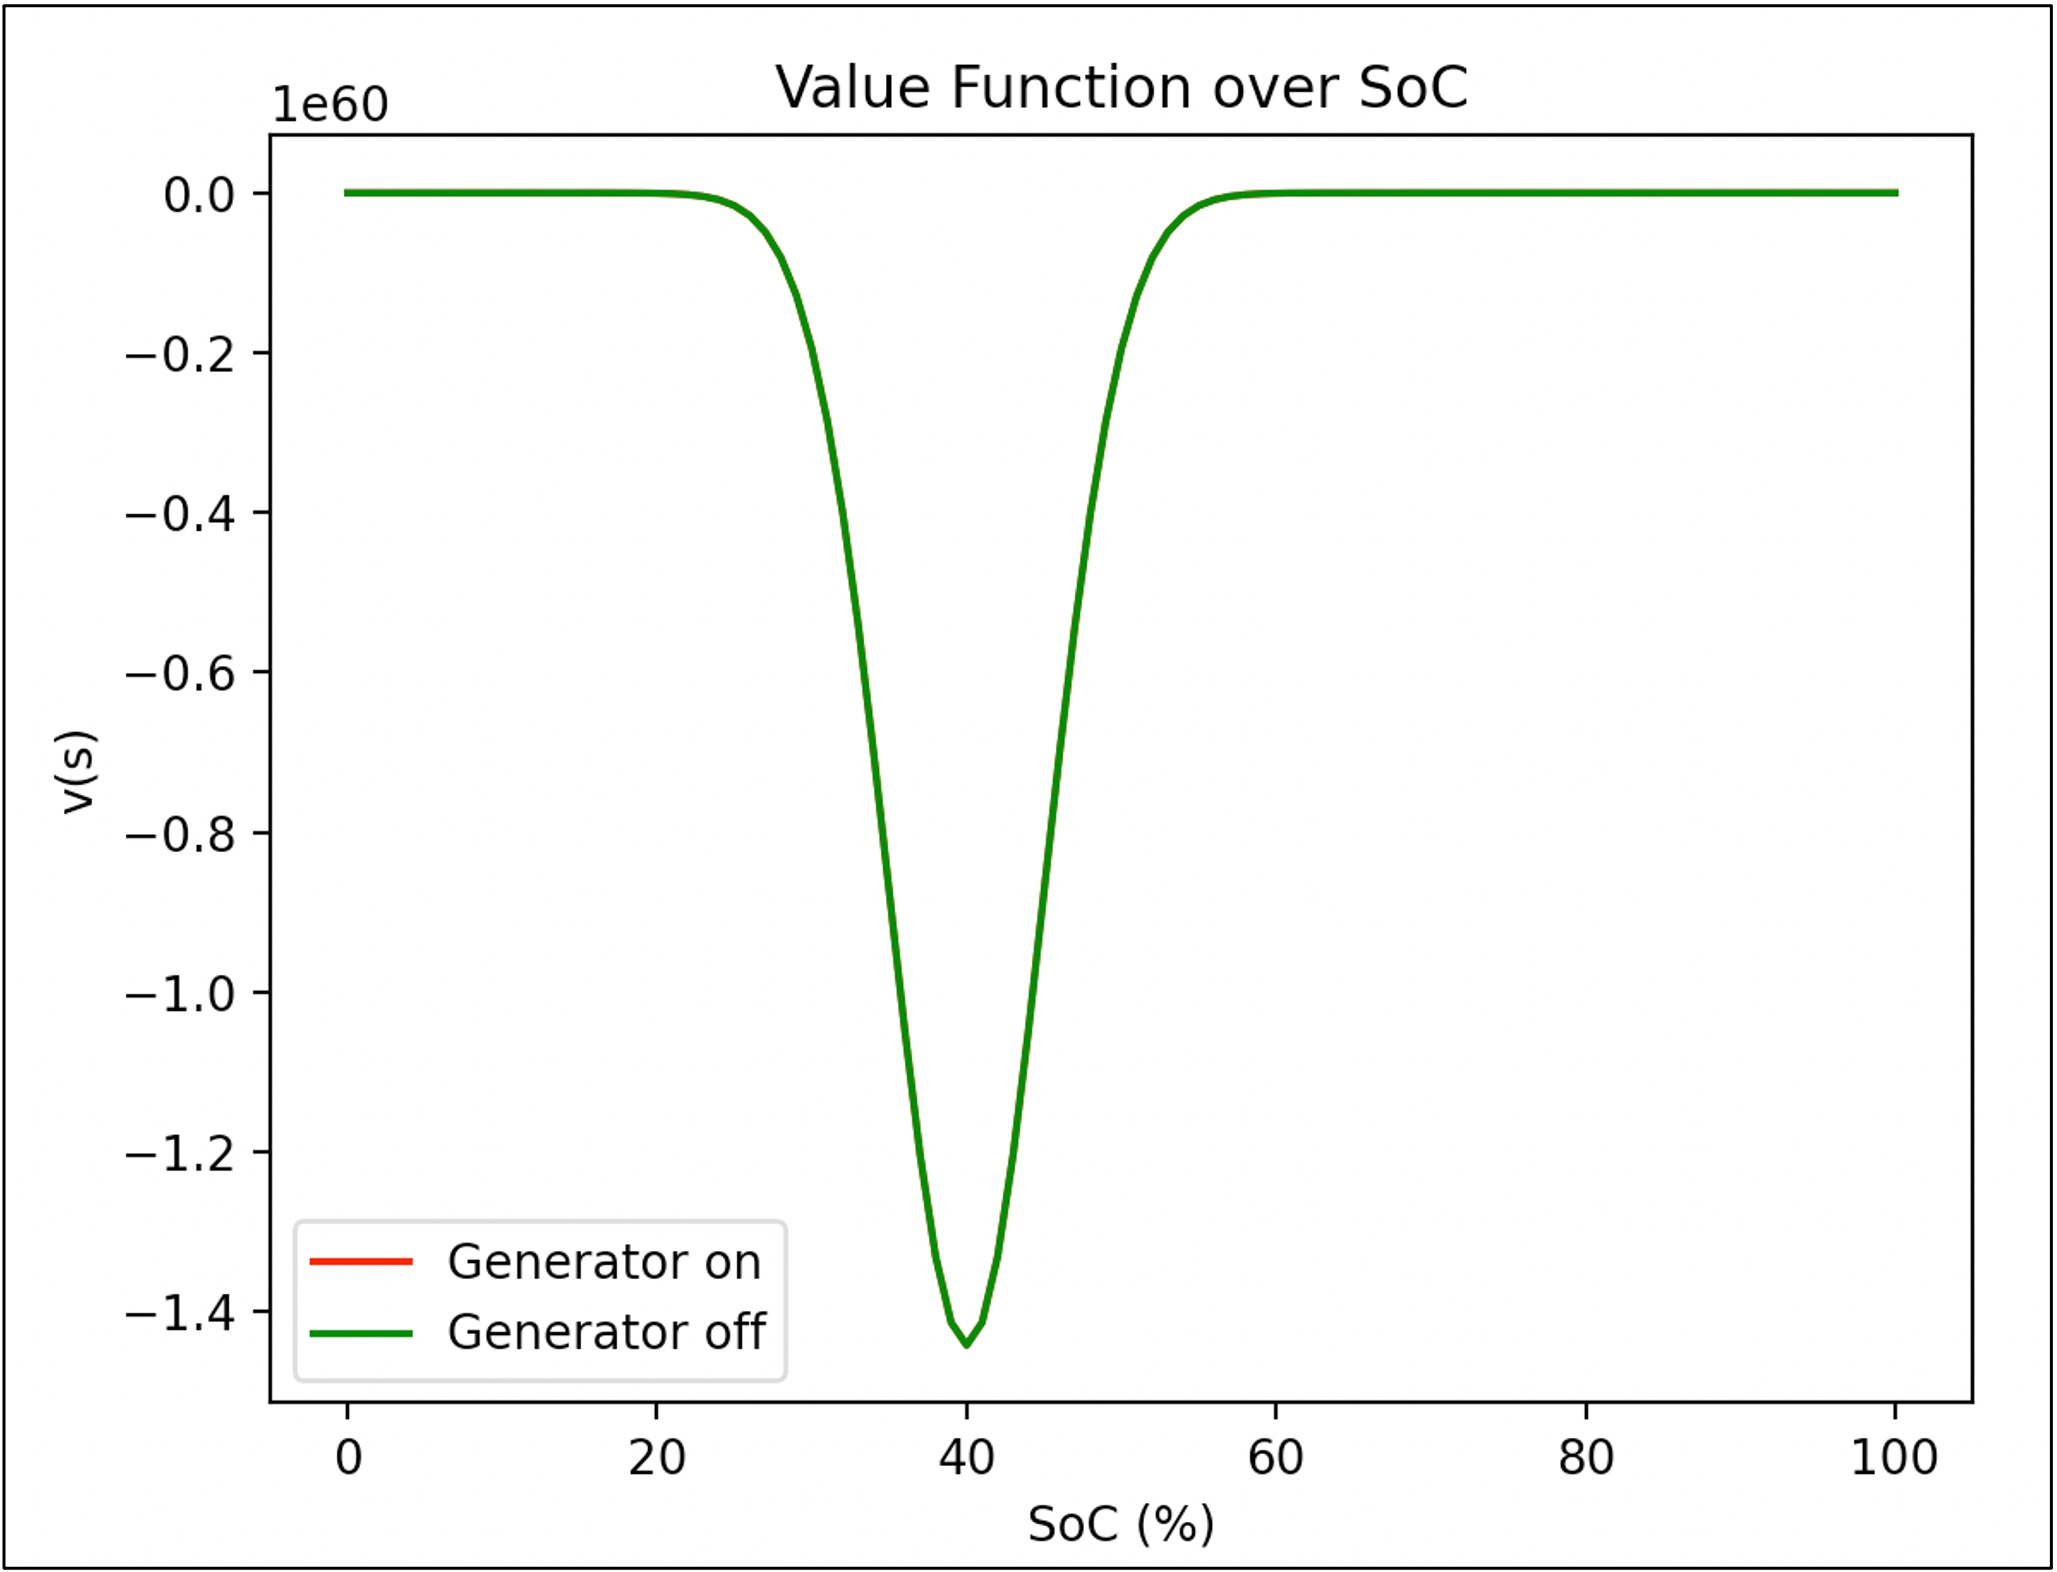
\includegraphics[width=\linewidth]{pics/rbfvaluefunc.jpg}
    \caption{Value function approximation}
  \end{subfigure}
  \begin{subfigure}[b]{0.3\linewidth}
    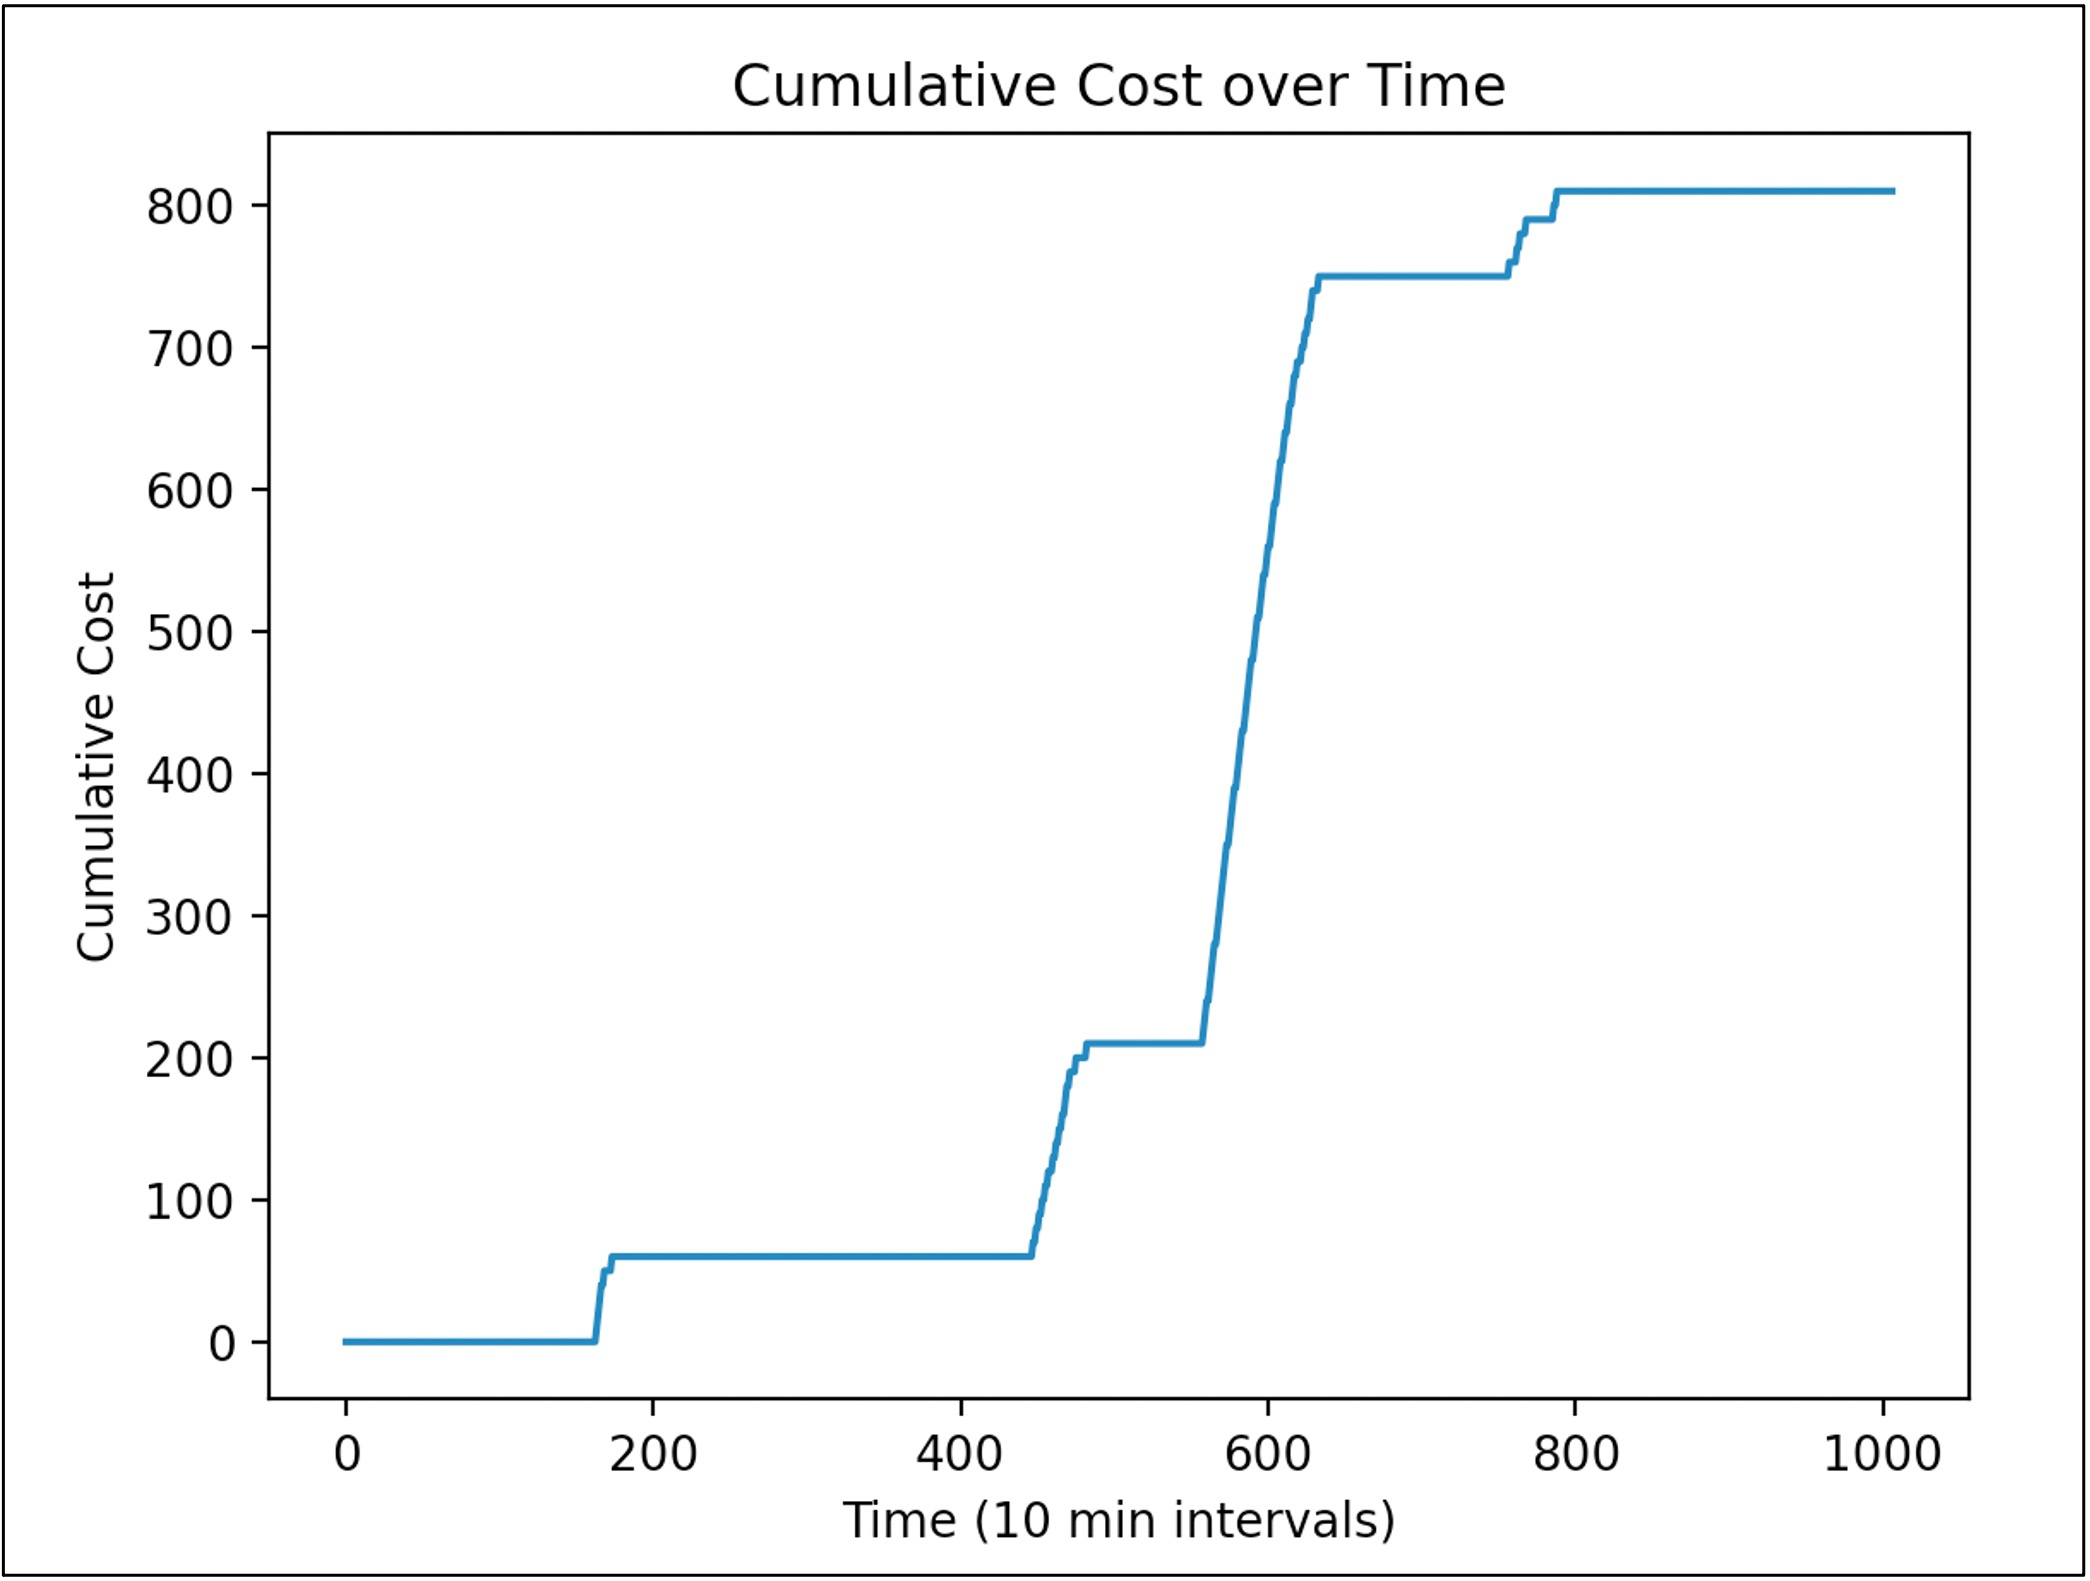
\includegraphics[width=\linewidth]{pics/rbfcostvtime.jpg}
    \caption{Cumulative cost over time}
  \end{subfigure}
  \caption{Graphs from the RBF model's policy}
  \label{fig:rbfgraphs}
\end{figure}


\section{Conclusion}
The results from this paper mirror those of the prior work. RL was an effective method for optimizing behavior in a smart grid setting. In simulations, the FVI model that approximated the value function as a linear spline performed the best and resulted in  more desirable results than the naive policy the SML currently uses. Ideally this modeling strategy could be expanded to include other areas of the SML and produce even more improvements. Expanding the model would also make integrating it into the real SML system easier. Other future work that could be done on the model is including prediction inputs for power generation and demand, or a time variable to help account for weather changes throughout the year. This could help improve the accuracy of the model because it would allow for a more detailed representation of seasons and the future. Another addition to the model could be to include a reward for having surplus energy, beyond what is needed to fully charge the battery. This could be of interest to the researchers at the SML and could drastically change the policy it produces. All of the code for this project can be found at \cite{github}.


\section{Acknowledgements}
The author would like to thank advisor Dr. Marek Petrik for his thorough guidance in creating and improving this work. Dr. Weiwei Mo and Roozbeh Ghasemi also had a big impact in the planning and creation of this project. Thank you for your assistance and feedback.



\bibliographystyle{ieeetr}
\bibliography{sample}

\end{document}